\section{Implementation and Experiments}
\label{sec:Experiments}

In this section, we discuss both qualitative and quantitative registration results of our ResNet-LDDMM on different datasets. We compare some of our results to those obtained using a Varifold-type LDDMM implementation \cite{charon2013varifold}. Next, we report evaluations and comparisons on the most recent SHREC datasets (SHREC'2019 in Sec.\ref{Sec:SHREC2019} and SHREC'2020 in Sec.\ref{Sec:SHREC2020}) and discuss strengths and limitations (Sec.\ref{Sec:limitations}). In the supplementary materials (SM), we discuss the influence of the regularization term, the impact of the network width, i.e. the parameter $m$ and the key role that the \textit{ReLU} activation function plays inside the building blocks $f^l$, as ablative studies. We compare the computational complexity of ResNet-LDDMM compared to LDDMM and existing approaches.  We also study the robustness of ResNet-LDDMM to noise and missing data.         

\subsection{Qualitative Comparison to LDDMM}
\label{sec:LDDMMcomparison}

Both LDDMM and ResNet-LDDMM produce a topology-preserving transformation (i.e. a diffeomorphism) of the whole ambient space $\real^3$. However, there are several differences between the two make the ResNet approach both easier to run and more adapted to certain problems, particularly those involving very distinct motions in different areas of the considered shape. This is because LDDMM methods require choosing a certain ``scale". For a discrete surface, when using a Gaussian kernel $K(x,y)=\exp(\frac{\Vert x-y\Vert_2}{2\mu^2})$, the scale is $\mu$, and every vector field generated will be a sum of Gaussian vector fields with fixed variance $\mu$, each centered at a point on the shape (see \cite{arguillere2016multipleshapes} for example). As a result, moving points within distances less than $\mu$ in different directions requires a lot of energy, so such movements generally do not appear when minimizing the functional Eq. (\ref{Eq:LDDMM}). However, the scale cannot be too small, or the motion will no longer need to preserve the topology of the triangulated surface. As a result, two main difficulties appear in LDDMM that the ResNet version improves upon. 

\begin{figure}[ht!]
  \centering
   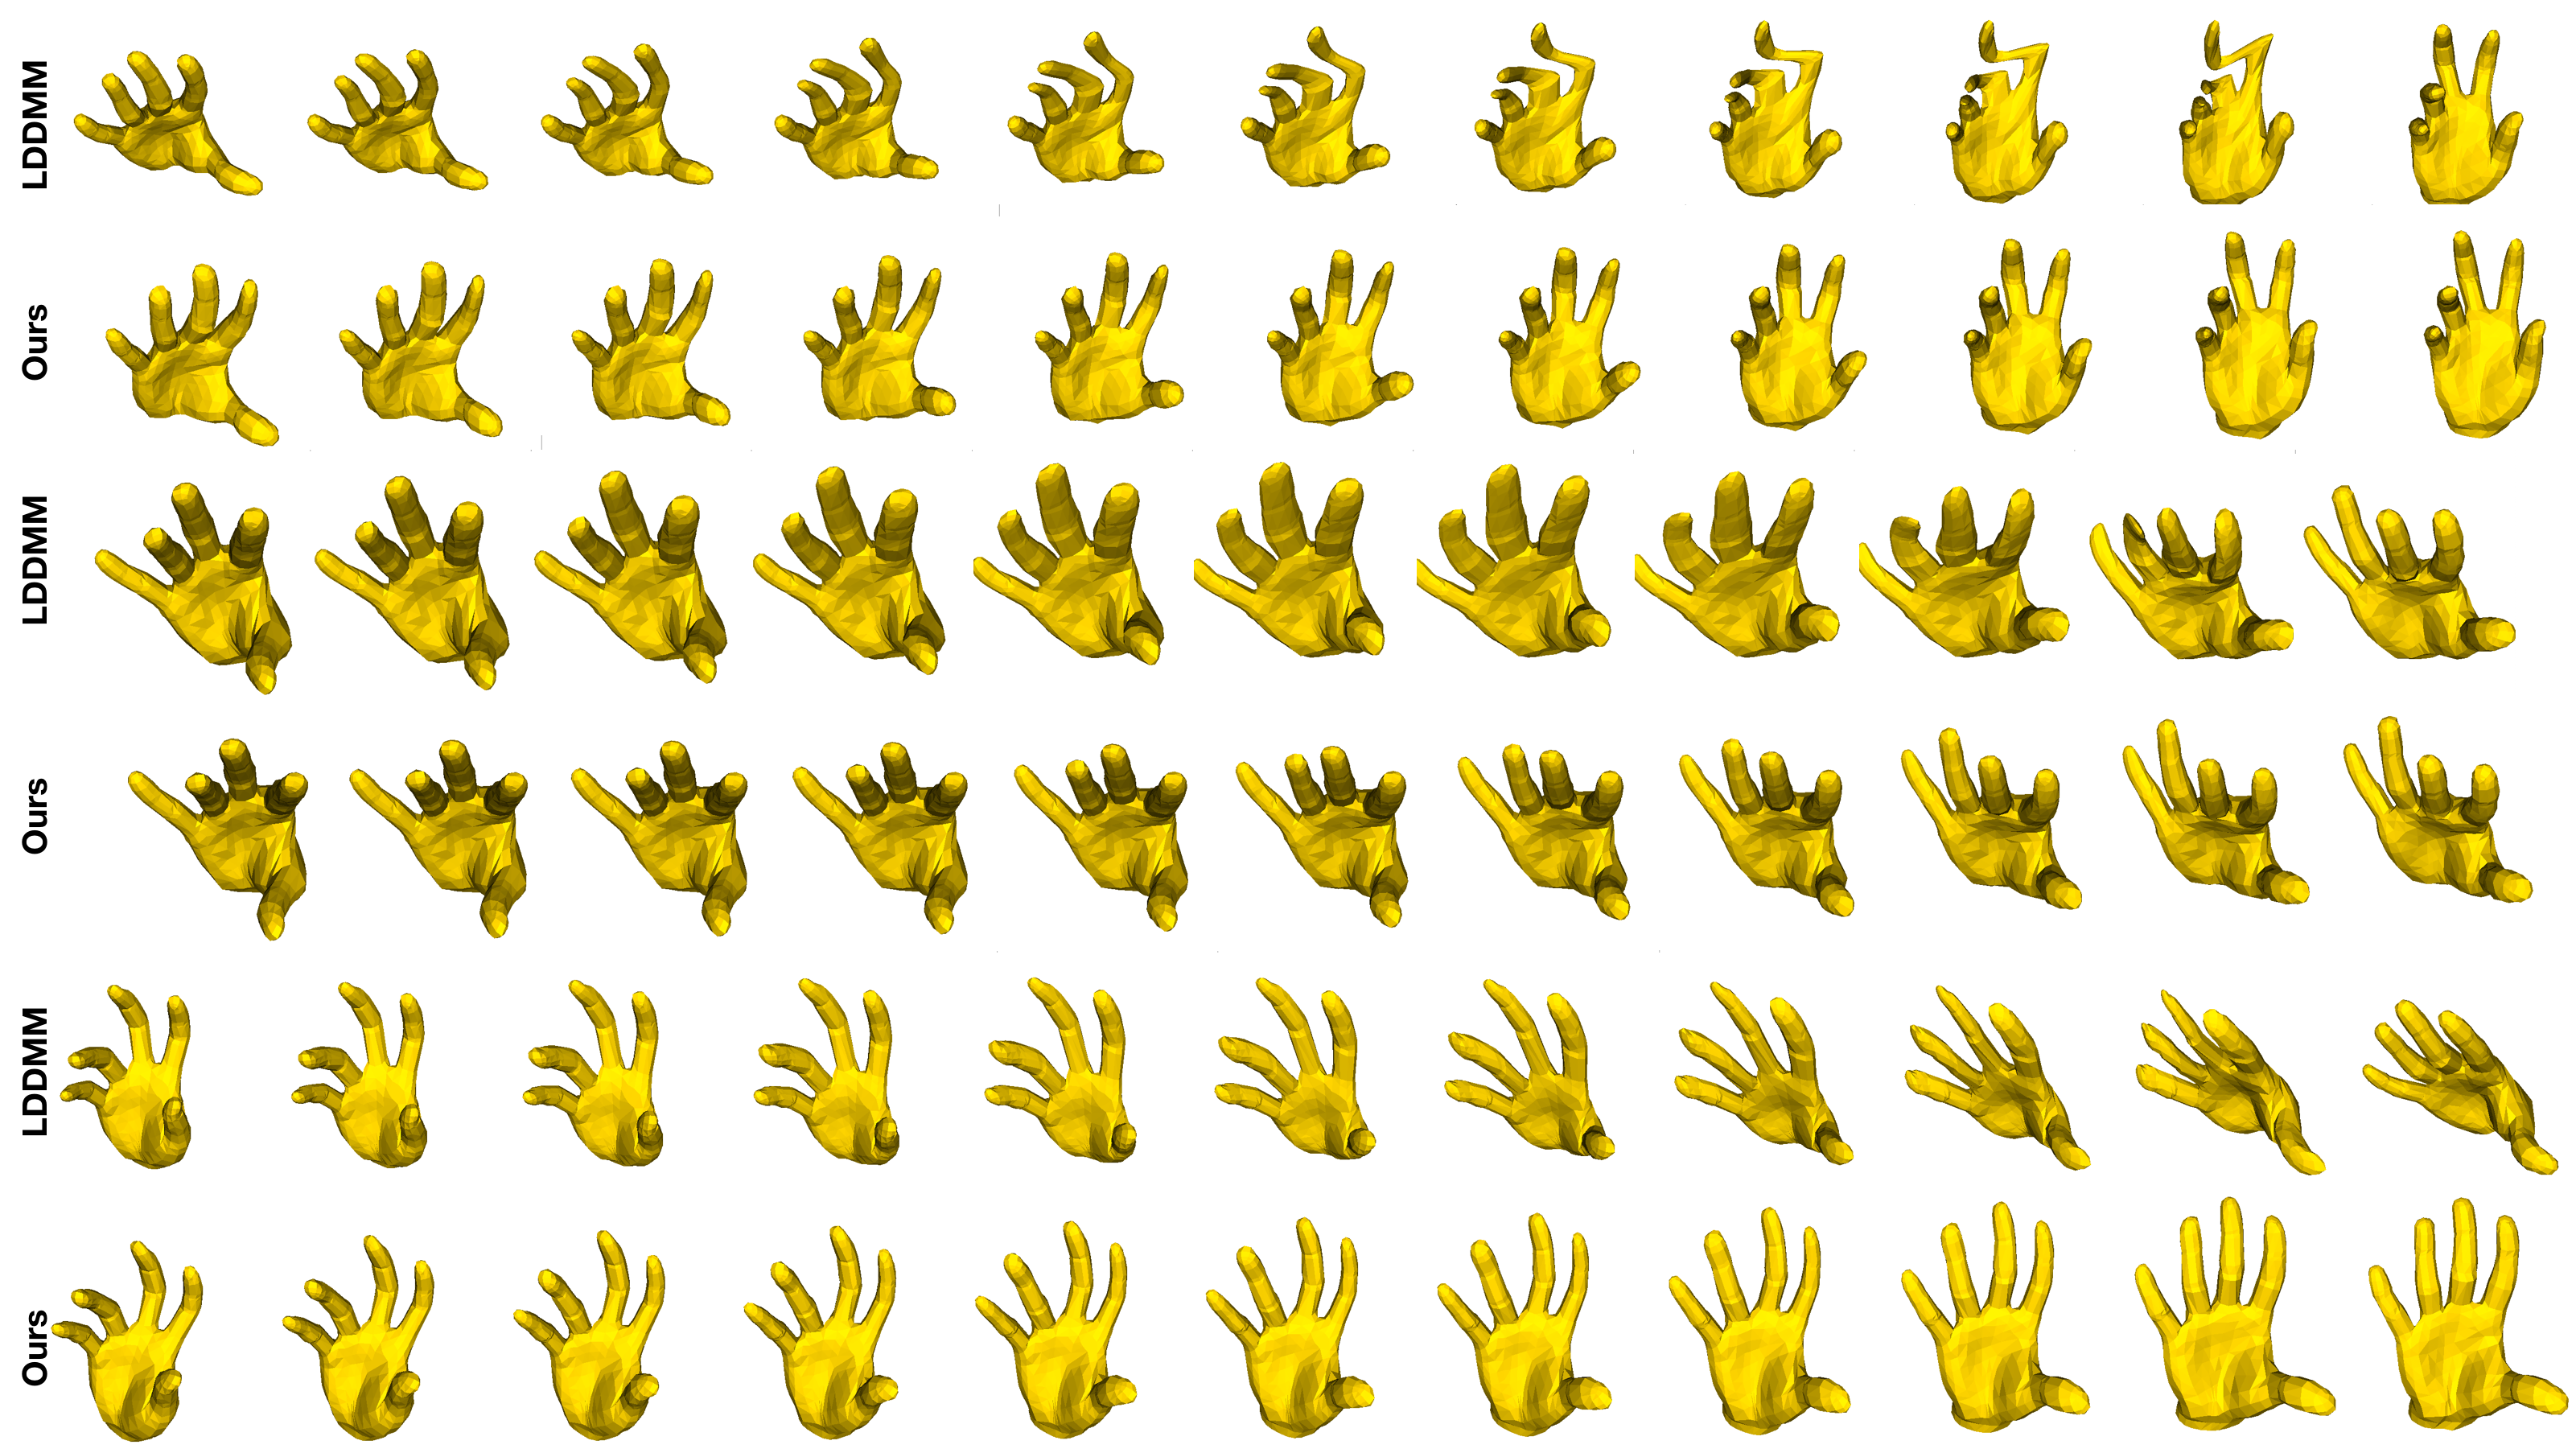
\includegraphics[width=1\linewidth]{Figs/ResNetvsLDMM.png}
    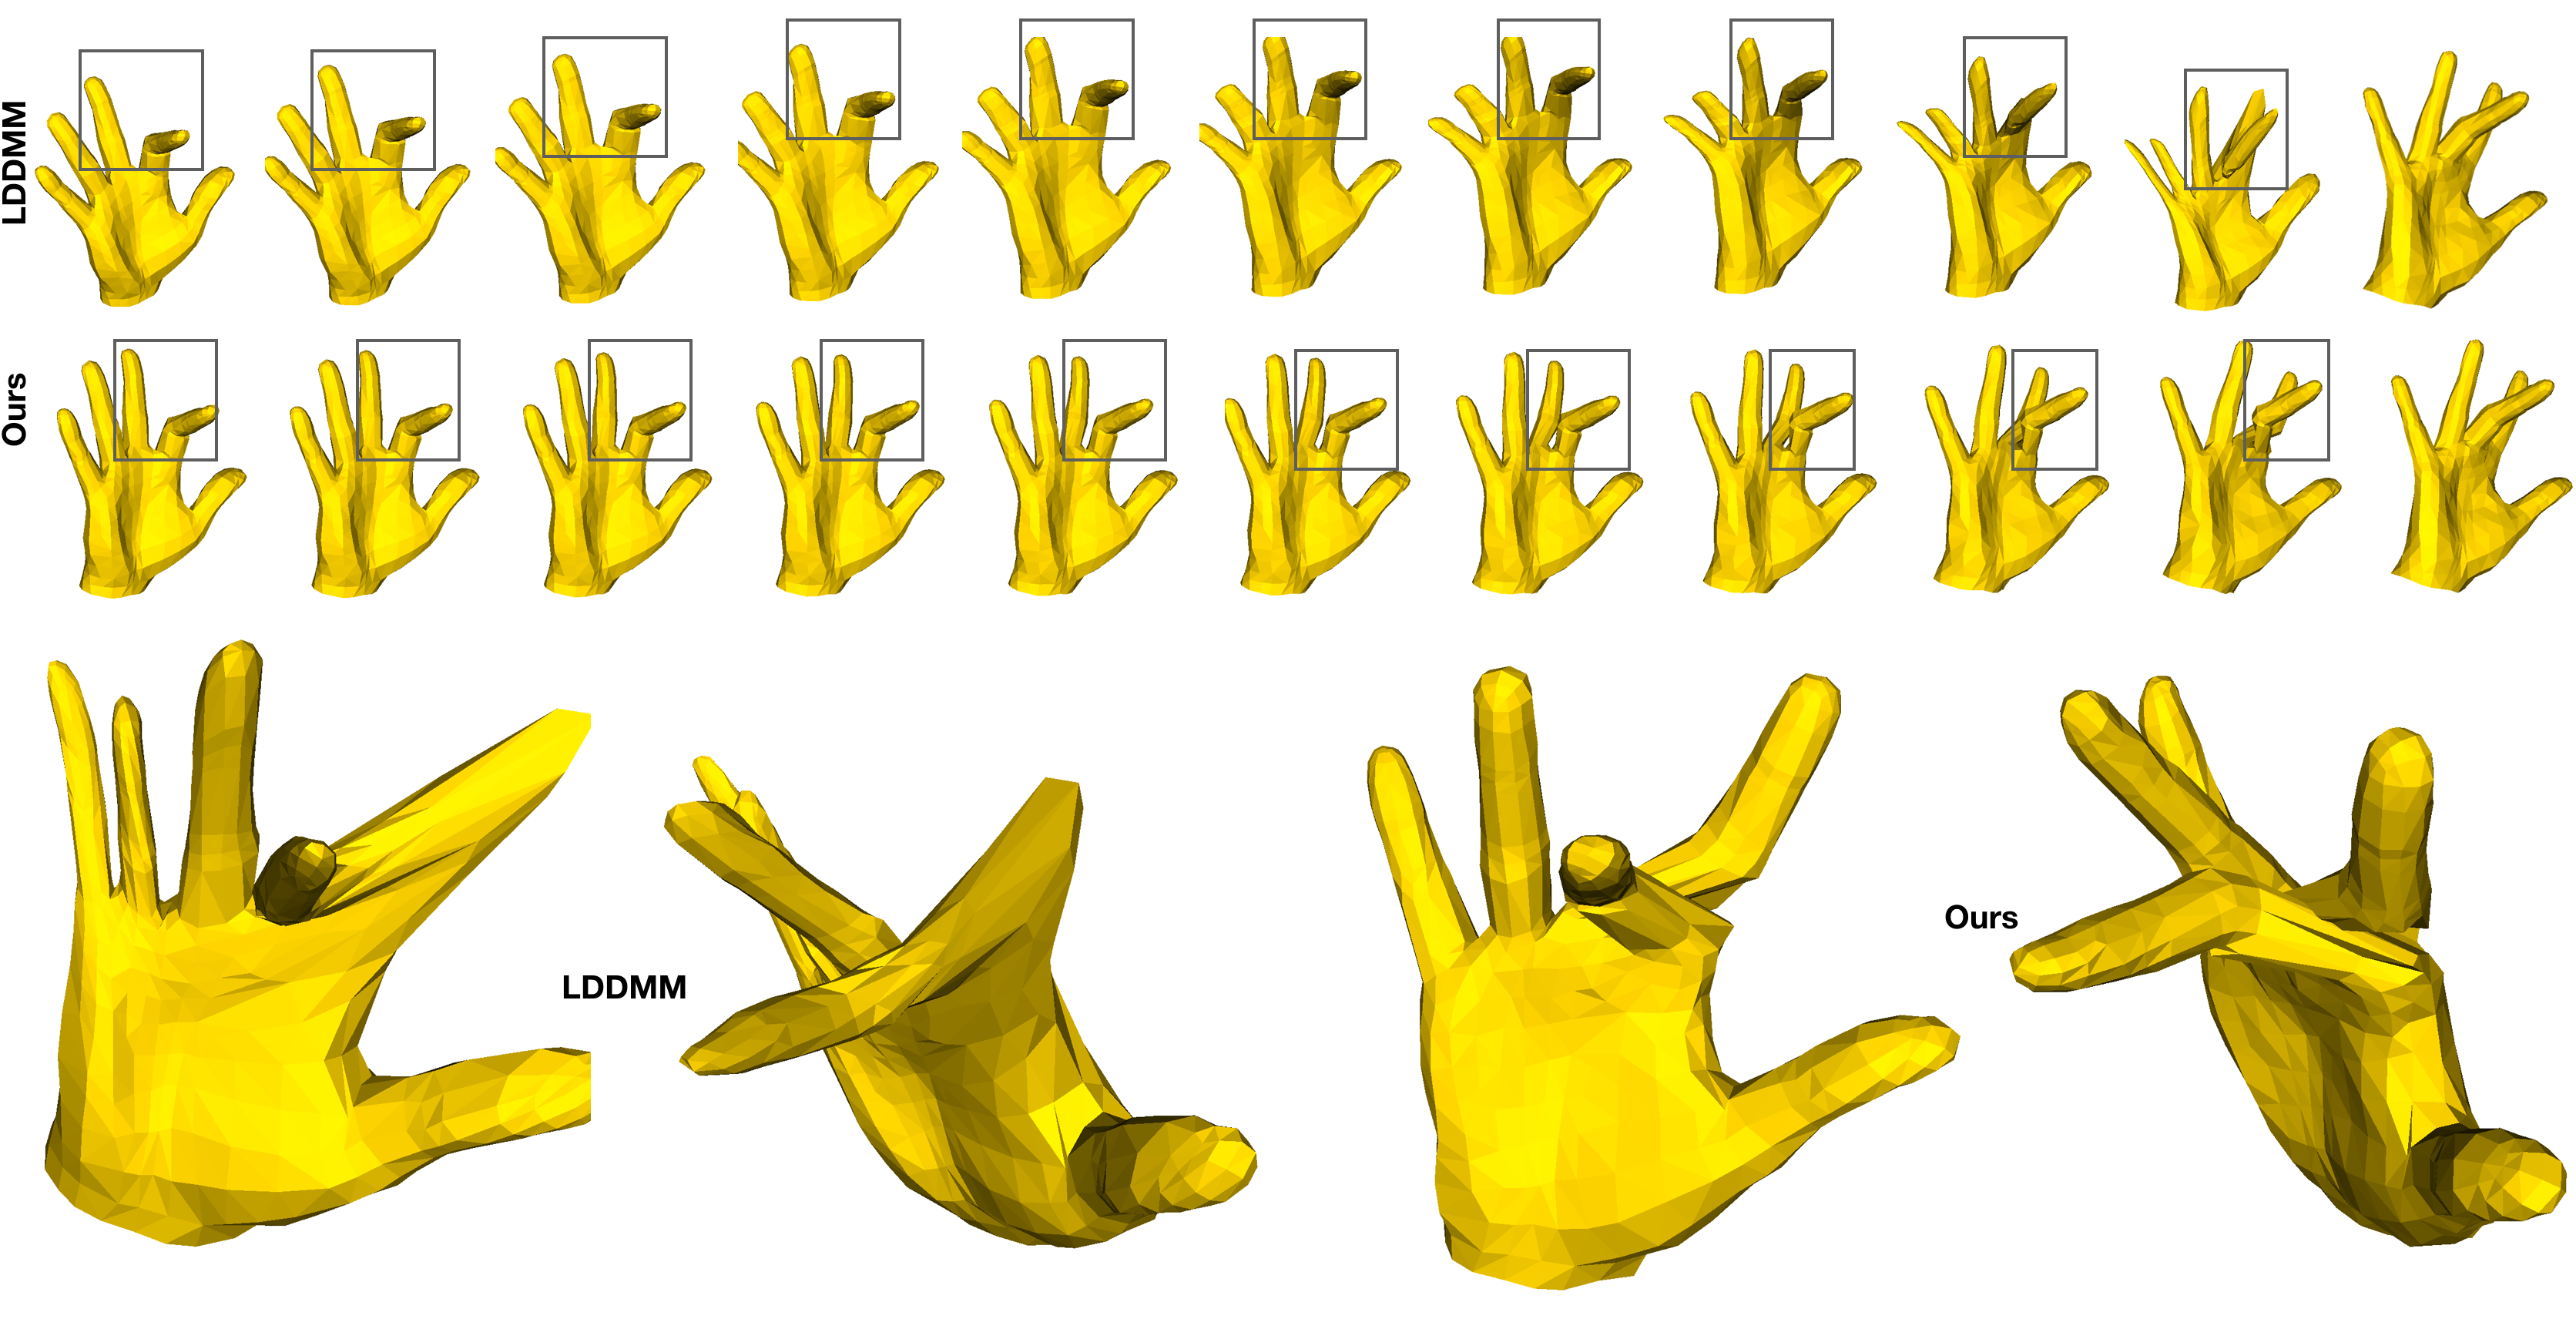
\includegraphics[width=\linewidth]{Figs/ResNetvsLDDMM-2.png}
    % \vspace{-0.8cm}
  \caption{Four examples to compare ResNet-LDDMM (ours) to LDDMM. }
   \label{Fig:ComparisonToLDDMM}
\end{figure}


\textbf{--} First, in LDDMM, one must find a ``good" scale $\mu$, which cannot be too small or too large, in order to allow a wide enough range of motions while still preserving the smoothness of the deformation. That is much less of a problem with ResNet-LDDMM: the size of the polytopes on which the velocity fields are computed not fixed, and so the algorithm automatically computes polytopes and polyhedrons of appropriate sizes. The role of scale falls instead on the width $m$ of the network. However, we will see that the results are not particularly sensitive to a change of width less than an order of magnitude, and simply choosing a width of a few hundred yielded good results on every case we tested. Further there is no automated way to find the best scale, so finding the correct one for LDDMM simply requires testing several values (with a bit of intuition to avoid bad ones). Hence, finding the best scale can sometimes take several days, and so we often settle one that is simply ``good enough". Whether the results of Tab. 2 of the Supplementary Materials are due to not finding the correct scale, or to our ResNet beating the best scale is up to debate, but regardless the ResNet results were obtained on the first try, which for practical applications is a clear improvement. %For synthetic heart, we report the results of rigid ICP instead of LDDMM as the high data resolution do not allow such simulations. 

\textbf{--} Second, there may not even be a good scale in the LDDMM framework to compare certain shapes. This is generally caused by points belonging to very different parts of the shape that also happen to be very close, such as two fingers on a hand. Such matching problems are generally much harder for the usual LDDMM, because one needs to choose big enough scales of deformation in the reproducing kernel to ensure regularity of the shape. This can either prevent necessary deformations from occurring, or force the transformation to first separate and unnaturally expand the fingers during the first half of the transformation. This is also a well-known problem when tackling multiple shapes (see \cite{arguillere2016multipleshapes} for example). This problem is particularly obvious in Fig. \ref{Fig:ComparisonToLDDMM} when matching various hand positions, especially (but not only) in the intermediate deformation steps. On the other hand, thanks in part to only requiring bi-lipshitz regularity, ResNet-LDDMM can move two parts of the shape (such as two fingers) in opposite directions while keeping the regularization term small by encasing each part within distinct polytopes. Fig. \ref{Fig:Directions} illustrates how ResNet-LDDMM performs better than LDDMM for the case of a hand.% That is, the True Registration Error (see Sec. \ref{sec:Experiments} for definition) is much lower, and the geodesic much more plausible in the case of ResNet-LDDMM compared to LDDMM. 

\textbf{--} As a final difference between the methods, LDDMM is quadratic with respect to the resolution (i.e., the number of points), and is notoriously time-consuming to run. While matching two shapes usually takes a  acceptable amount of time, matching hundreds (or even thousands) for adequate statistical analysis can quickly become impossible. Significant advances have been made using GPUs and the free library KeOps (www.kernel-operations.io) on this front \cite{charlier2020kernel}, but it is still time-consuming to perform such an analysis, especially when one needs several retries to find the correct scales for the reproducing kernel. On the other hand, ResNet-LDDMM is much faster (refer to Supplementary Materials), especially at high resolution; the network itself actually has linear complexity with respect to the resolution. Only the data attachment terms have quadratic complexity. Combined with the lack of needing compute a correct scale, this new method seems like a clear winner in this area (at least for more than a few hundred points).% Tab. \ref{tab:LDDMMvsResNetLDDMM} summarizes the key differences between LDDMM and ResNet-LDDMM.

\subsection{Experiments on SHREC'2019}
\label{Sec:SHREC2019}

The SHREC'2019 dataset (Task.8) consists of articulated wooden mannequins and wooden hands. The organizers have created clothes for the models from two materials; one that can bend but is resistant to stretching, and another that can bend and stretch. To induce greater non-isometry, they used plasticine underneath the clothing of the model \cite{dyke2019shrec}. Because the dataset consists of real-world scans, it contains geometric inconsistencies and topological change caused by self-contact. The real-scans also contain natural noise, varying triangulation of shapes and occluded geometry. Four test sets have been released as follows: Test-set0 contains 14 pairs of articulating wooden hand objects; Test-set1 contains 26 pairs of models, comprising clothed humans and hands (limited to near-isometric deformations); Test-set2 contains 19 pairs of models; the pairings are between a thin clothed mannequin and a larger mannequin, ensuring significant non-isometry; Test-set3 contains 17 carefully selected pairs that contain challenging geometric and topological changes. 

\begin{figure}[ht!]
  \centering
   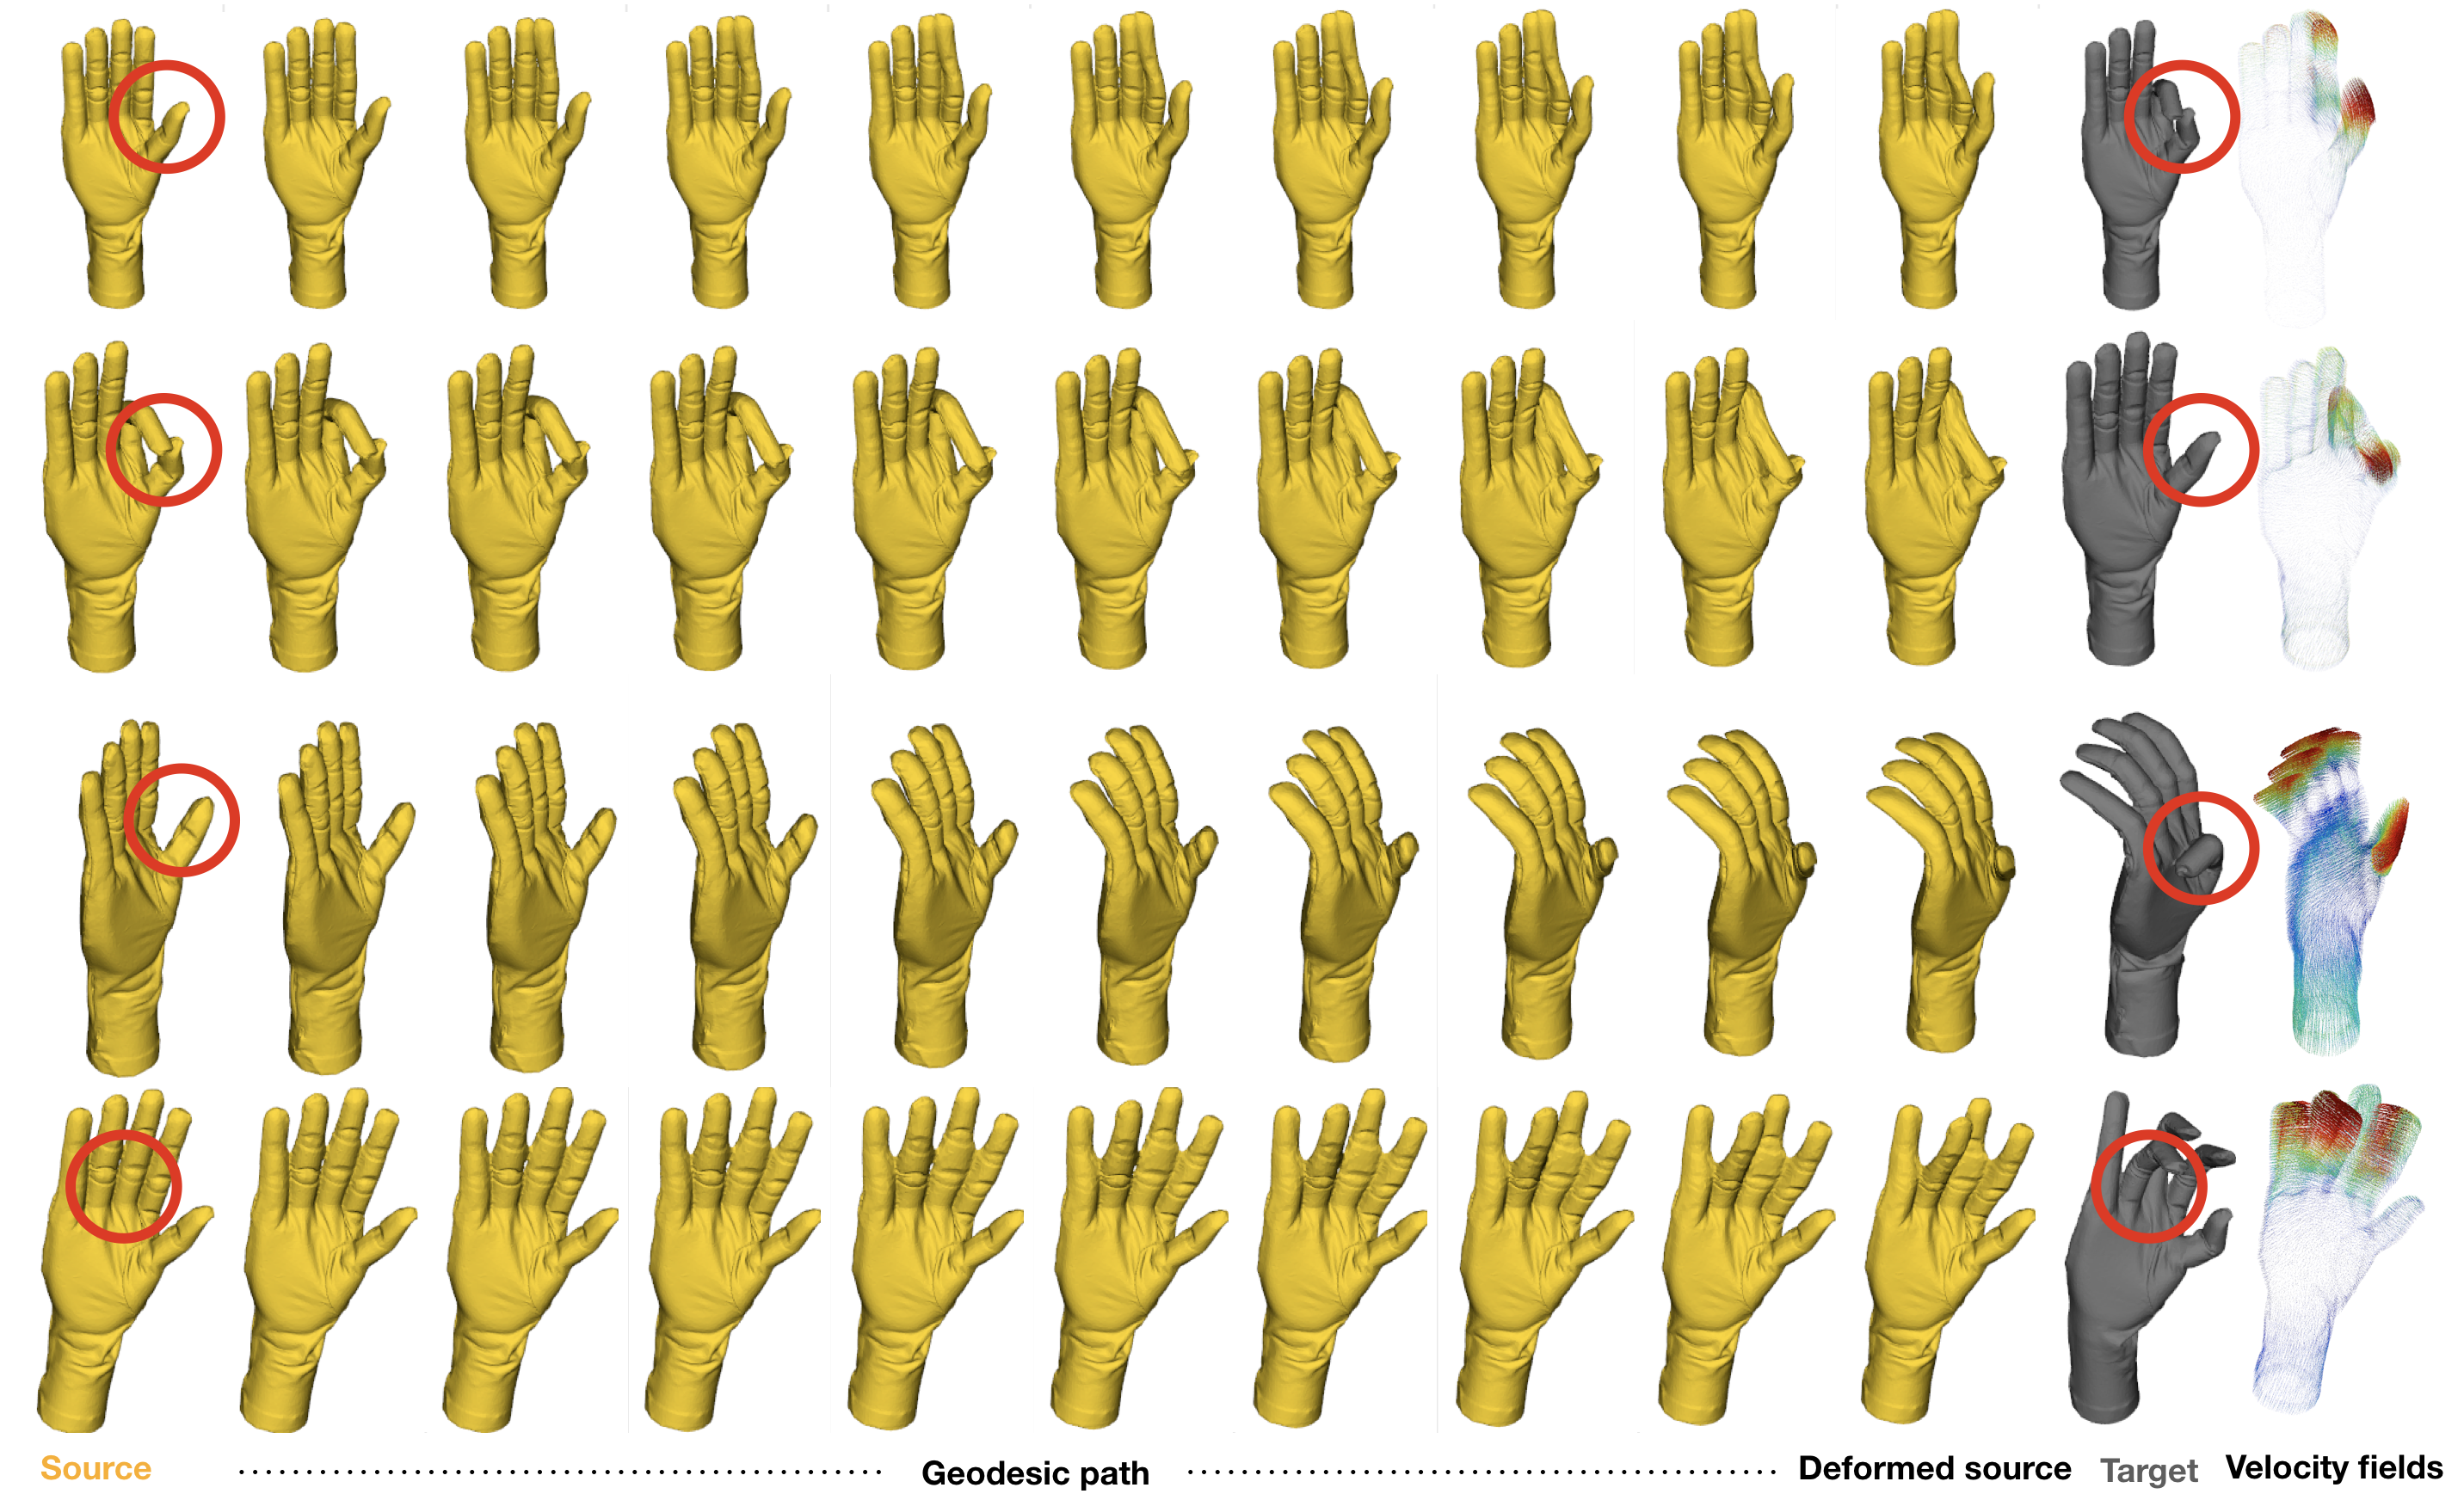
\includegraphics[width=1\linewidth]{Figs/TopologyExamples.png}
  \caption{Deformable registration achieved by ResNet-LDDMM (geodesic paths and computed velocity fields): Difficult examples where source and target shapes have different topology (highlighted in red circles).}
   \label{Fig:TopologyExamples}
\end{figure}

Results and comparison with existing methods are reported in Fig.\ref{Fig:SHREC2019}. We notice that only Dyke \etal \cite{dyke2019non} (and ours) have reported dense registration results. Also, while the majority of approaches start from an initial correspondence (based on SHOT descriptors) along with the diffusion pruning framework, our approach doesn't require such initialization. Finally, unlike the 3D-CODED approach \cite{groueix20183d}, tested only on test-set2 (human-like articulated mannequin), which requires a huge amount of data to train the network, ResNet-LDDMM is completely unsupervised. It is clear from these results (the fourth column, results on test-set3, reflects clearly this issue) the limitation of our ResNet-LDDMM to handle topological changes between the source and target shape. That is expected as, following LDDMM, ResNet-LDDMM was designed to compute a topology-preserving transformation. Examples reported in Fig.\ref{Fig:TopologyExamples} illustrate this limitation of our ResNet-LDDMM. 

\begin{figure*}[ht!]
  \centering
   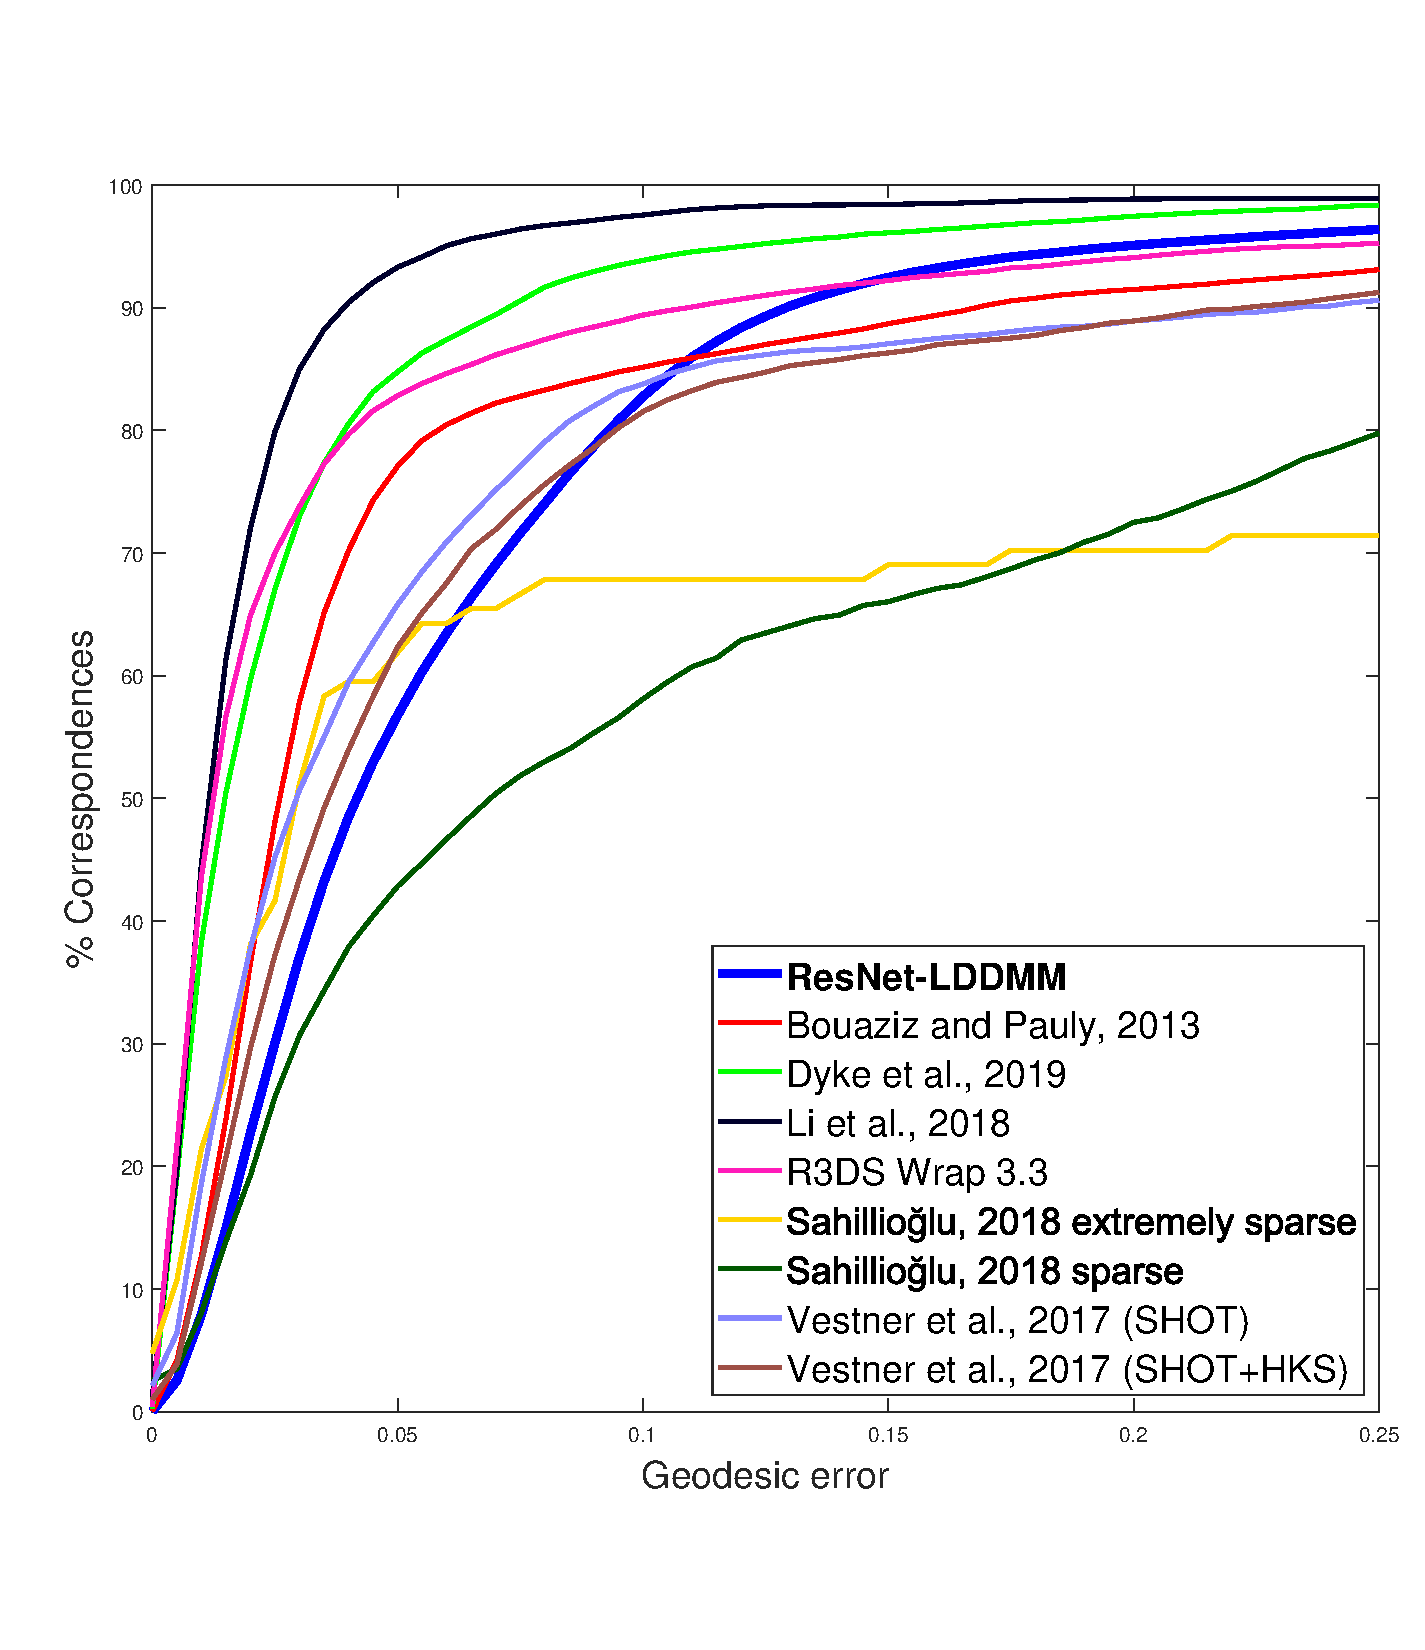
\includegraphics[width=.19\linewidth]{Figs/test-set0.pdf}
   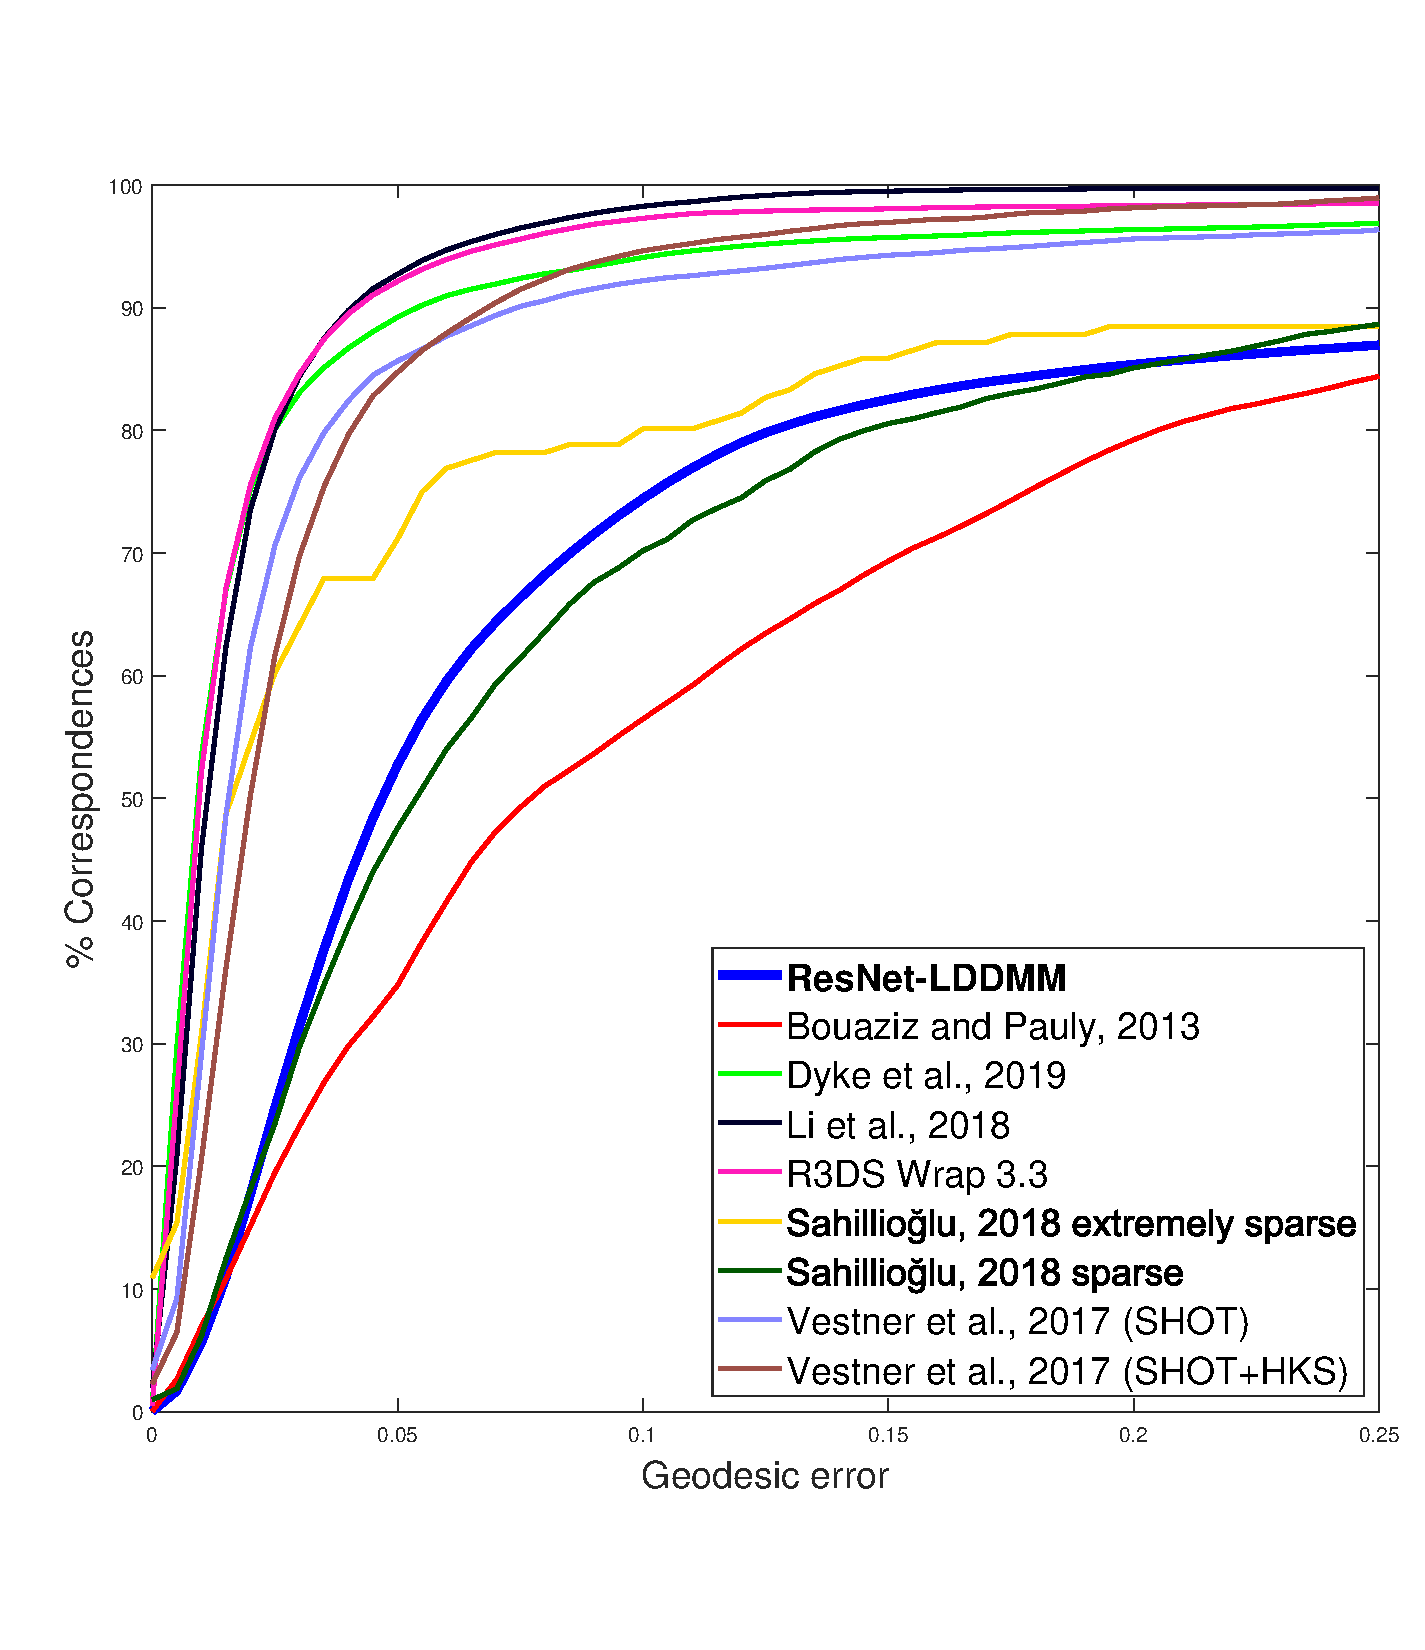
\includegraphics[width=.19\linewidth]{Figs/test-set1.pdf}
    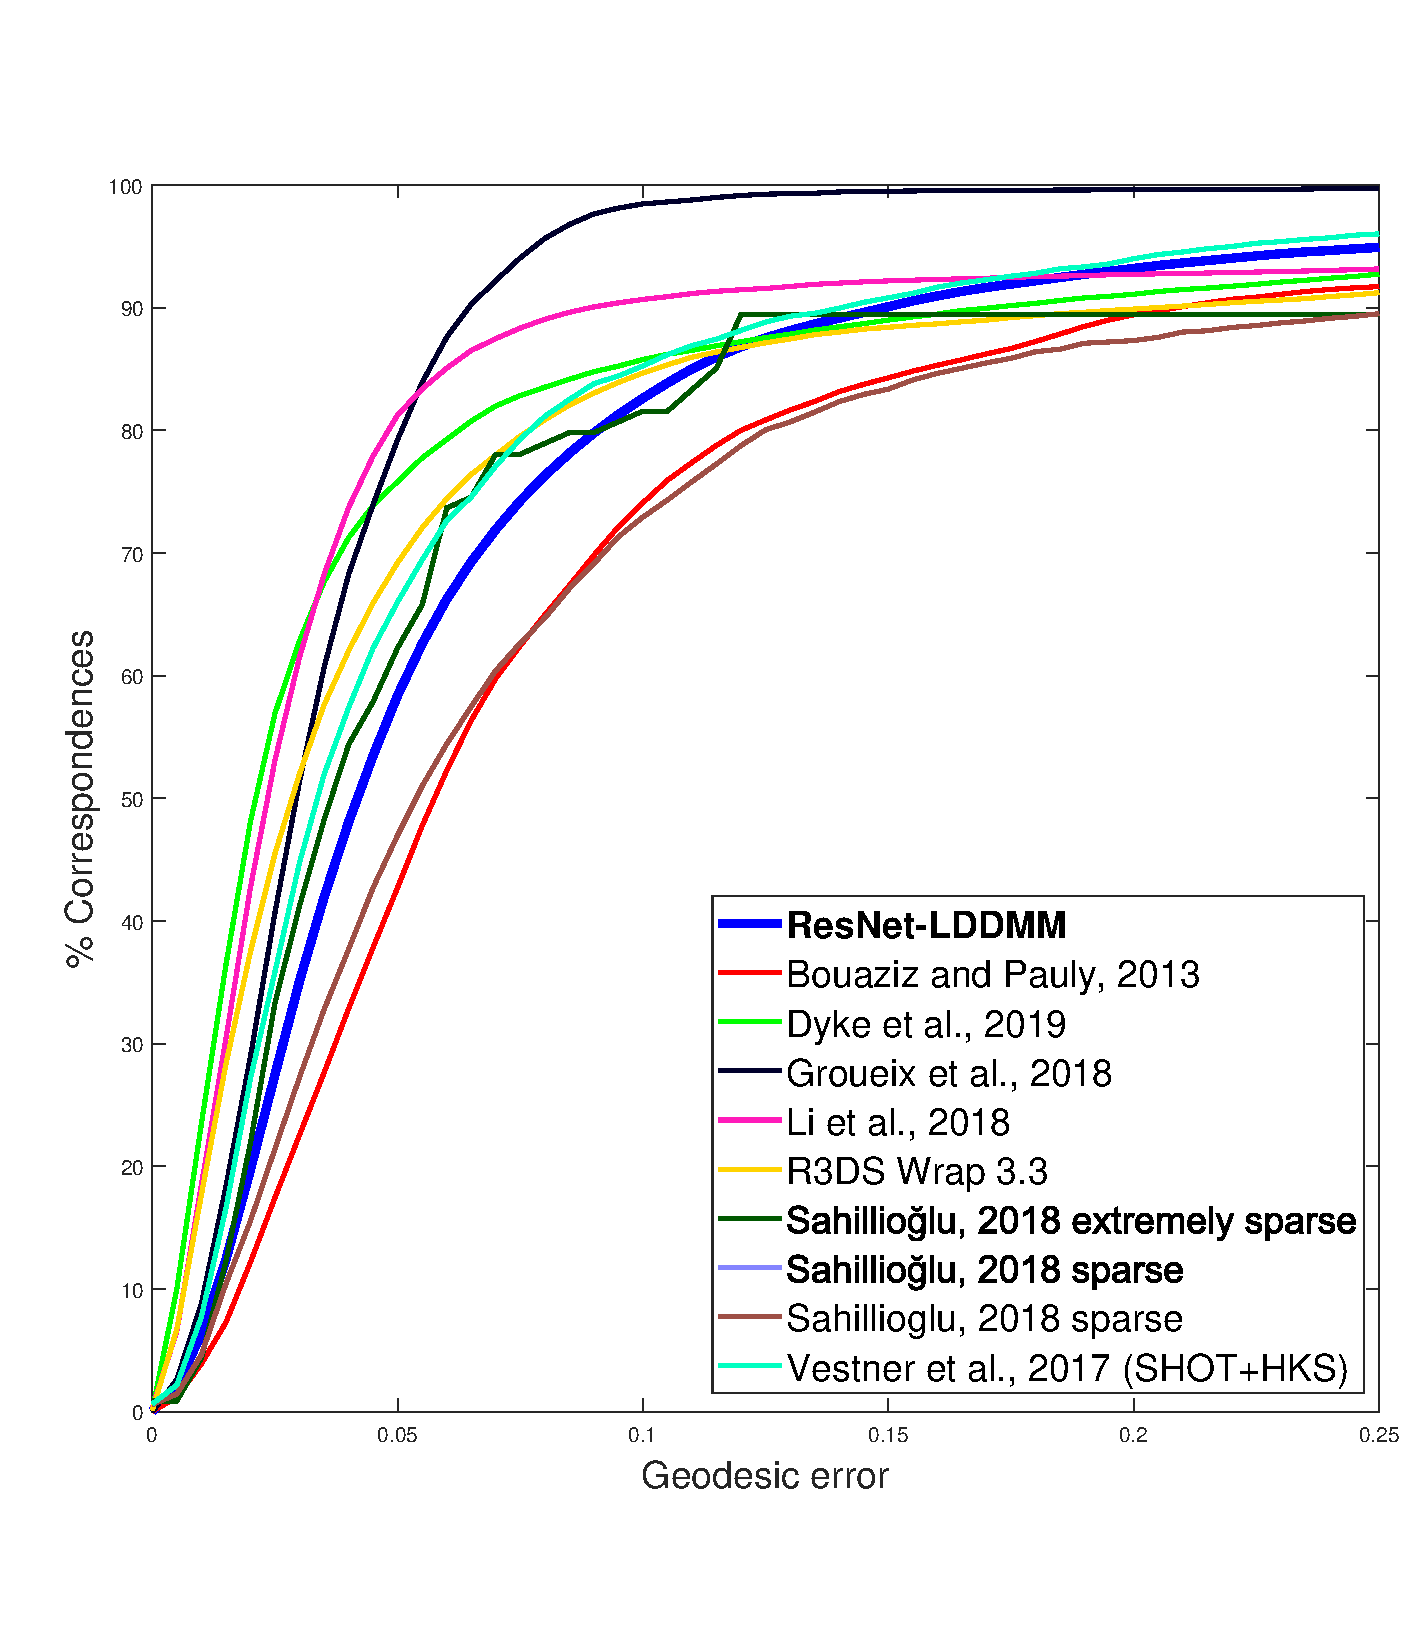
\includegraphics[width=.19\linewidth]{Figs/test-set2.pdf}
   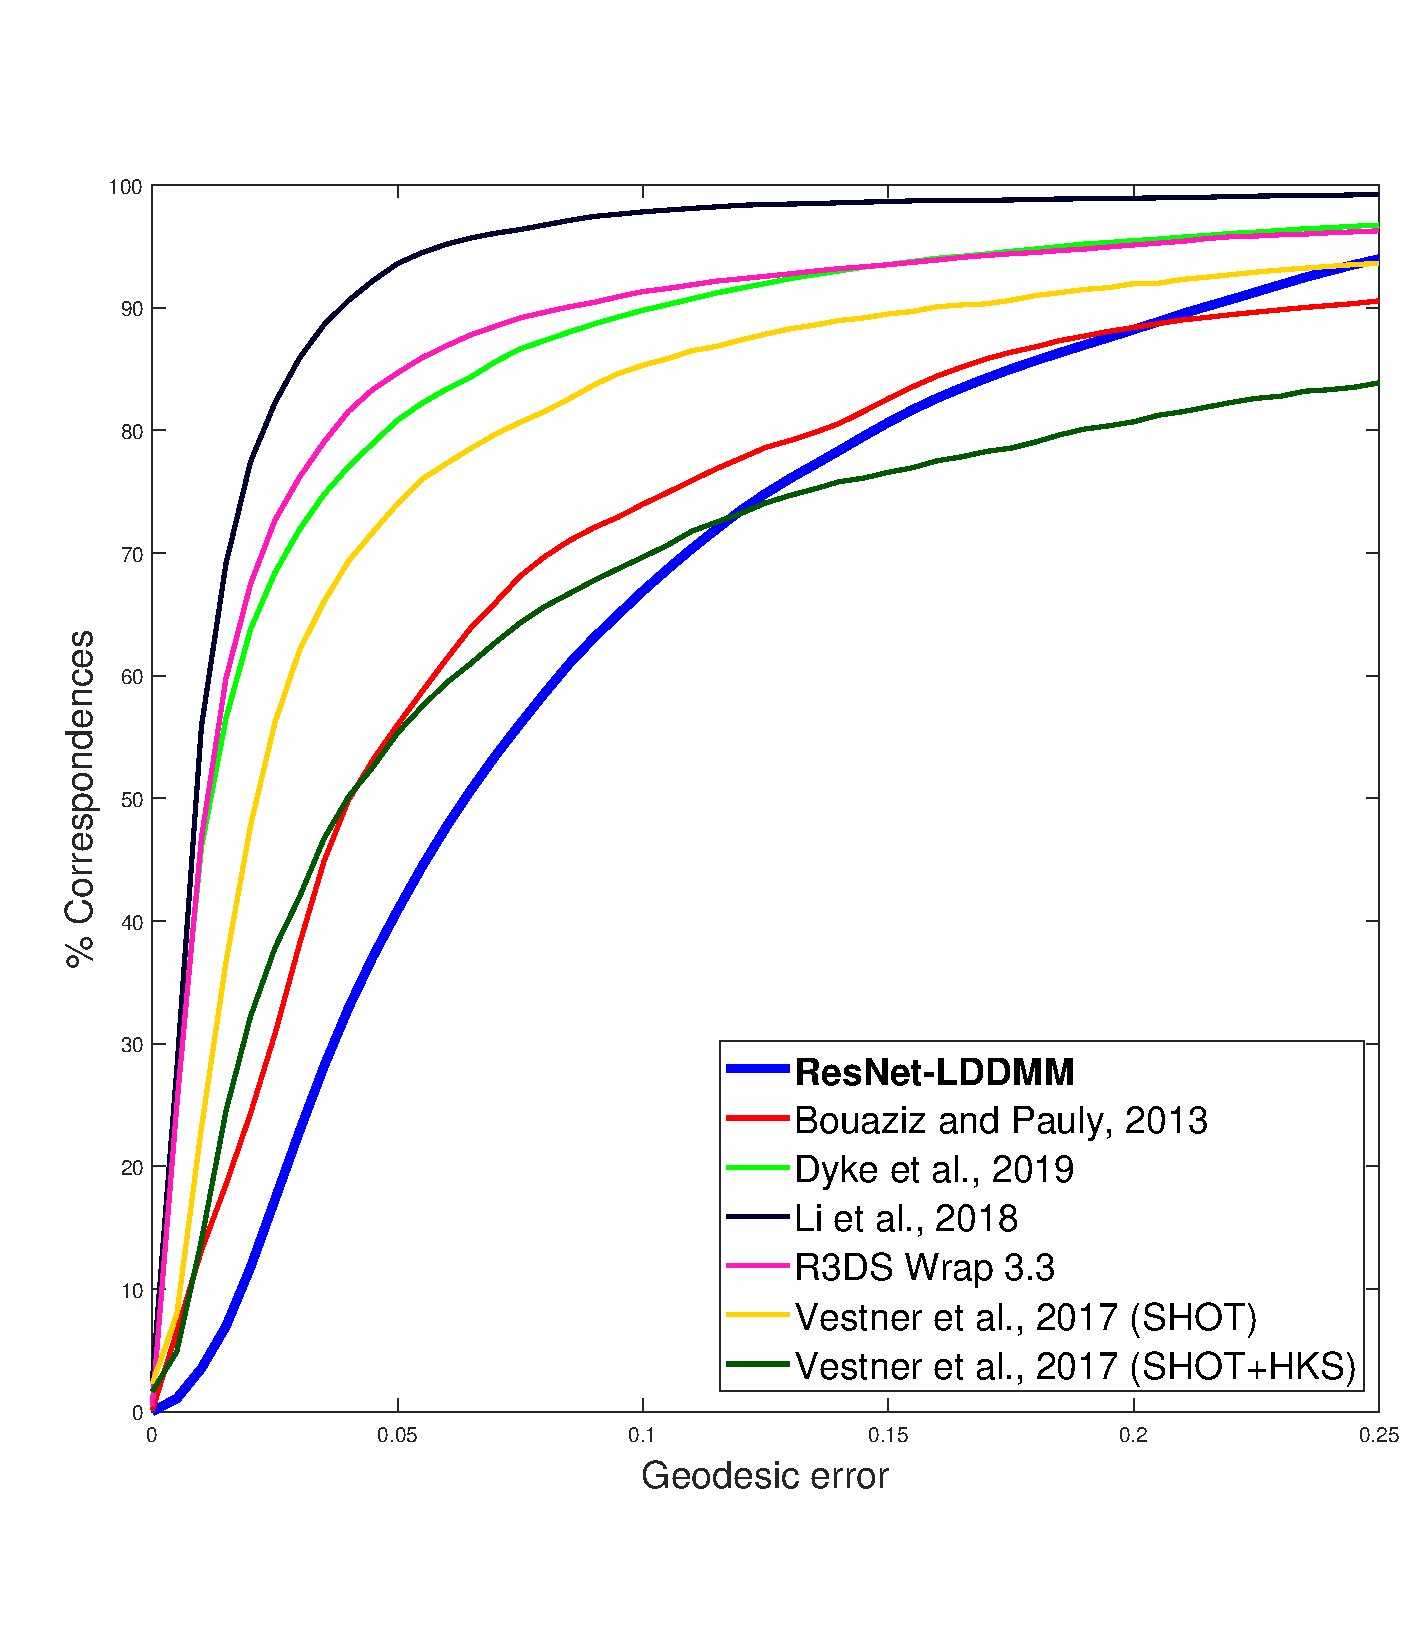
\includegraphics[width=.19\linewidth]{Figs/test-set3.pdf}
      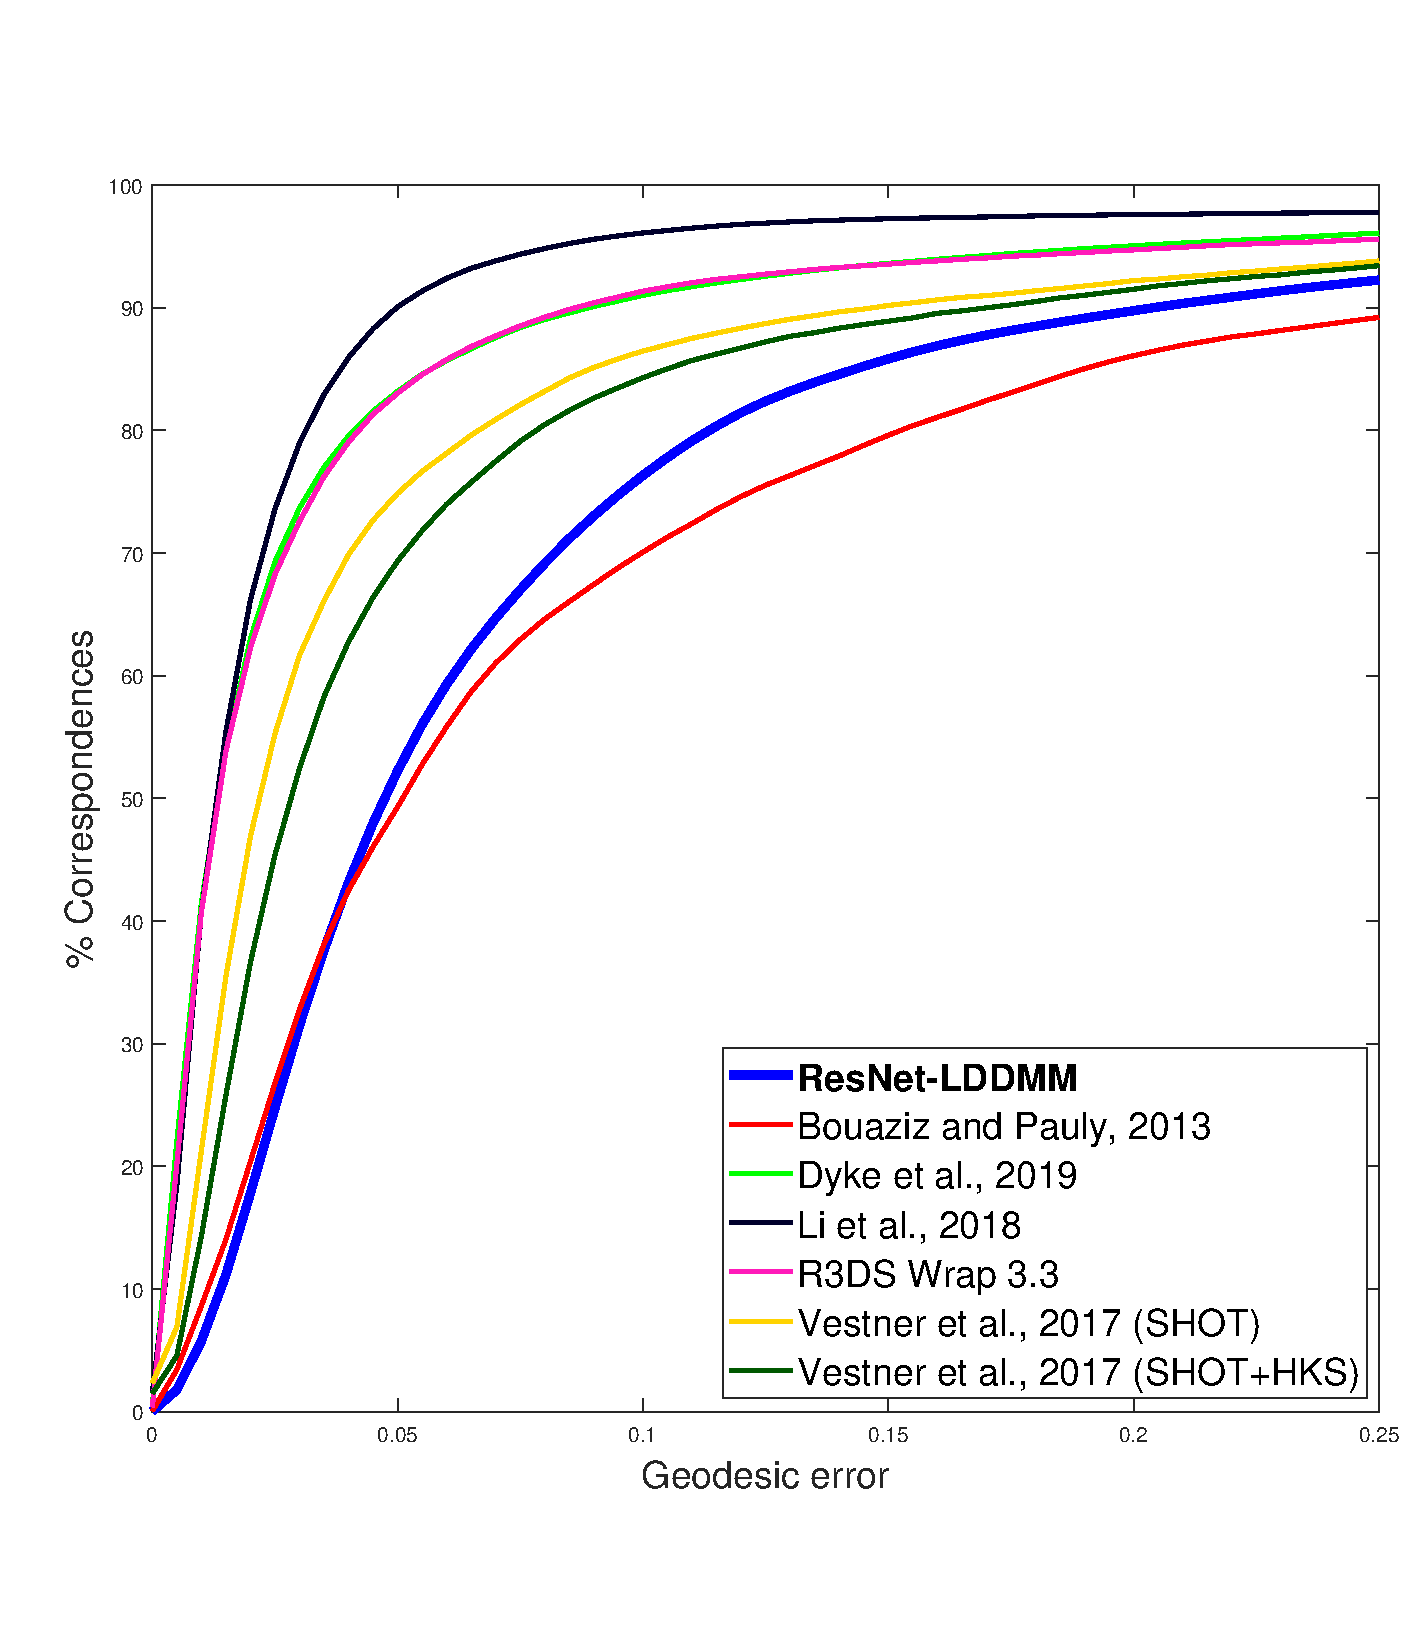
\includegraphics[width=.19\linewidth]{Figs/test-set-all.pdf}
        \vspace{-0.3cm}
\caption{Evaluation on SHREC'2019 and comparison with existing methods (from \cite{dyke2019shrec}). From left to right : test-set0 (articulated deformations), test-set1 (near-isometric deformations), test-set2 (non-isometric deformations), test-set3 (topological and geometric changes), all test-sets.}
   \label{Fig:SHREC2019}
\end{figure*}

\begin{figure*}[ht!]
  \centering
    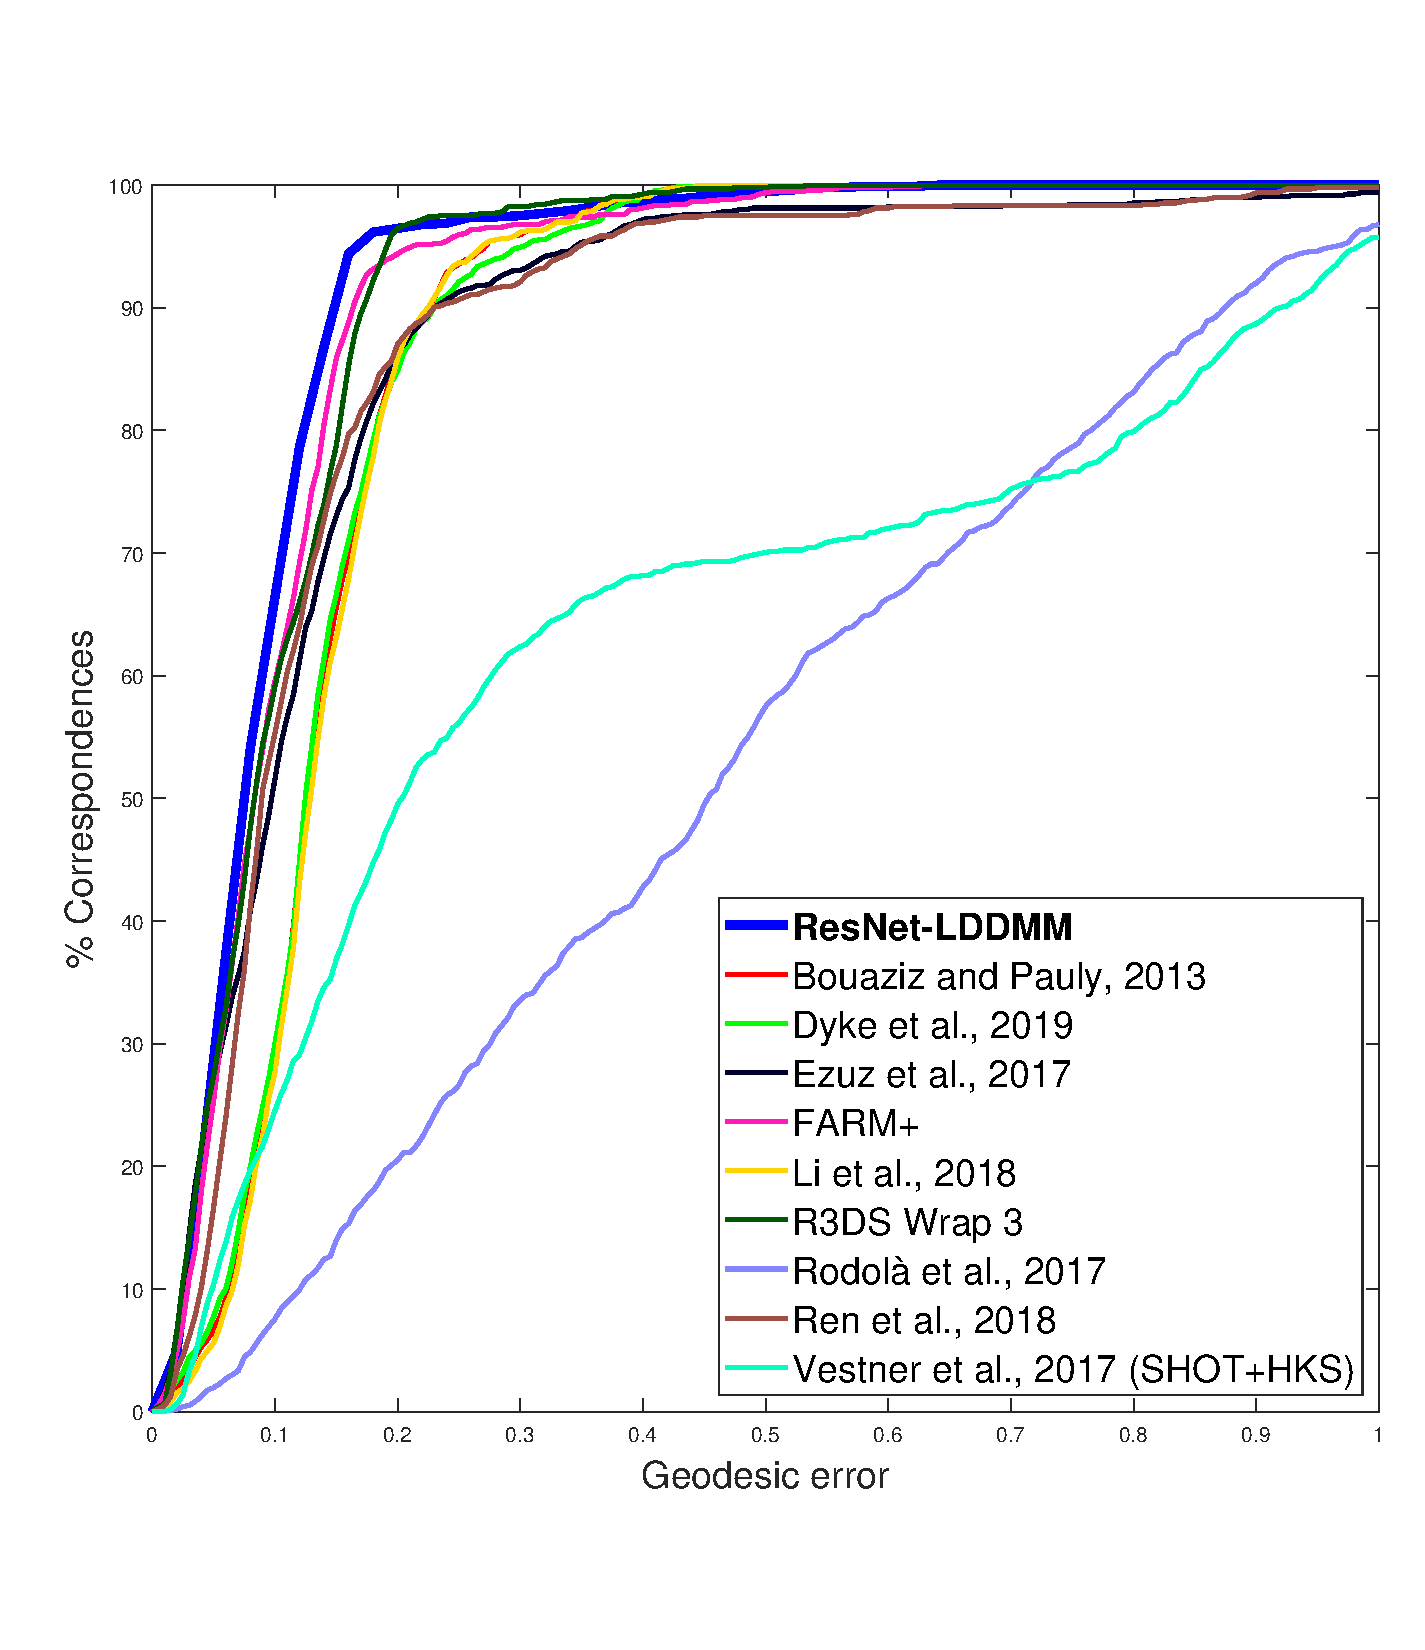
\includegraphics[width=0.19\linewidth]{Figs/7a.pdf}
    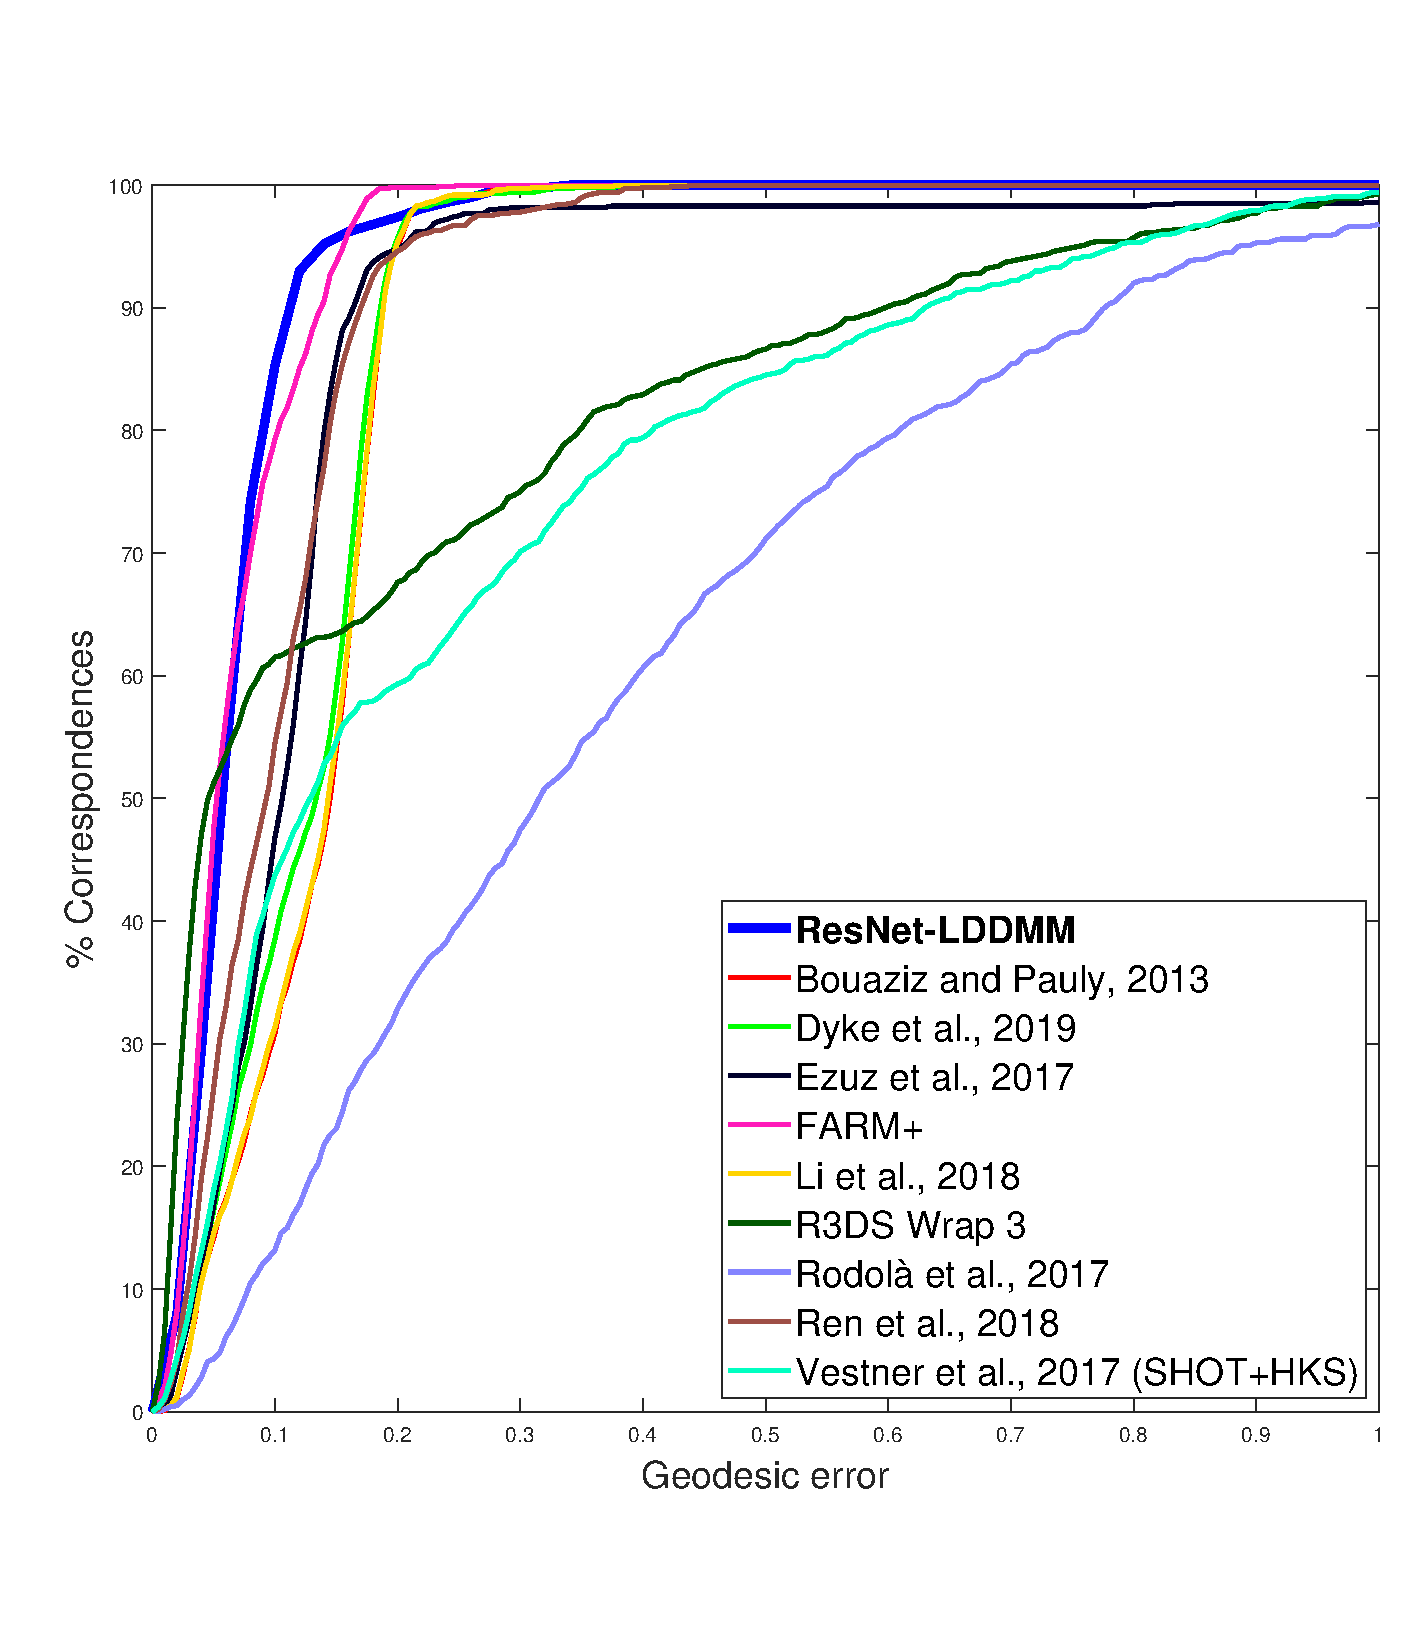
\includegraphics[width=0.19\linewidth]{Figs/7b.pdf}
    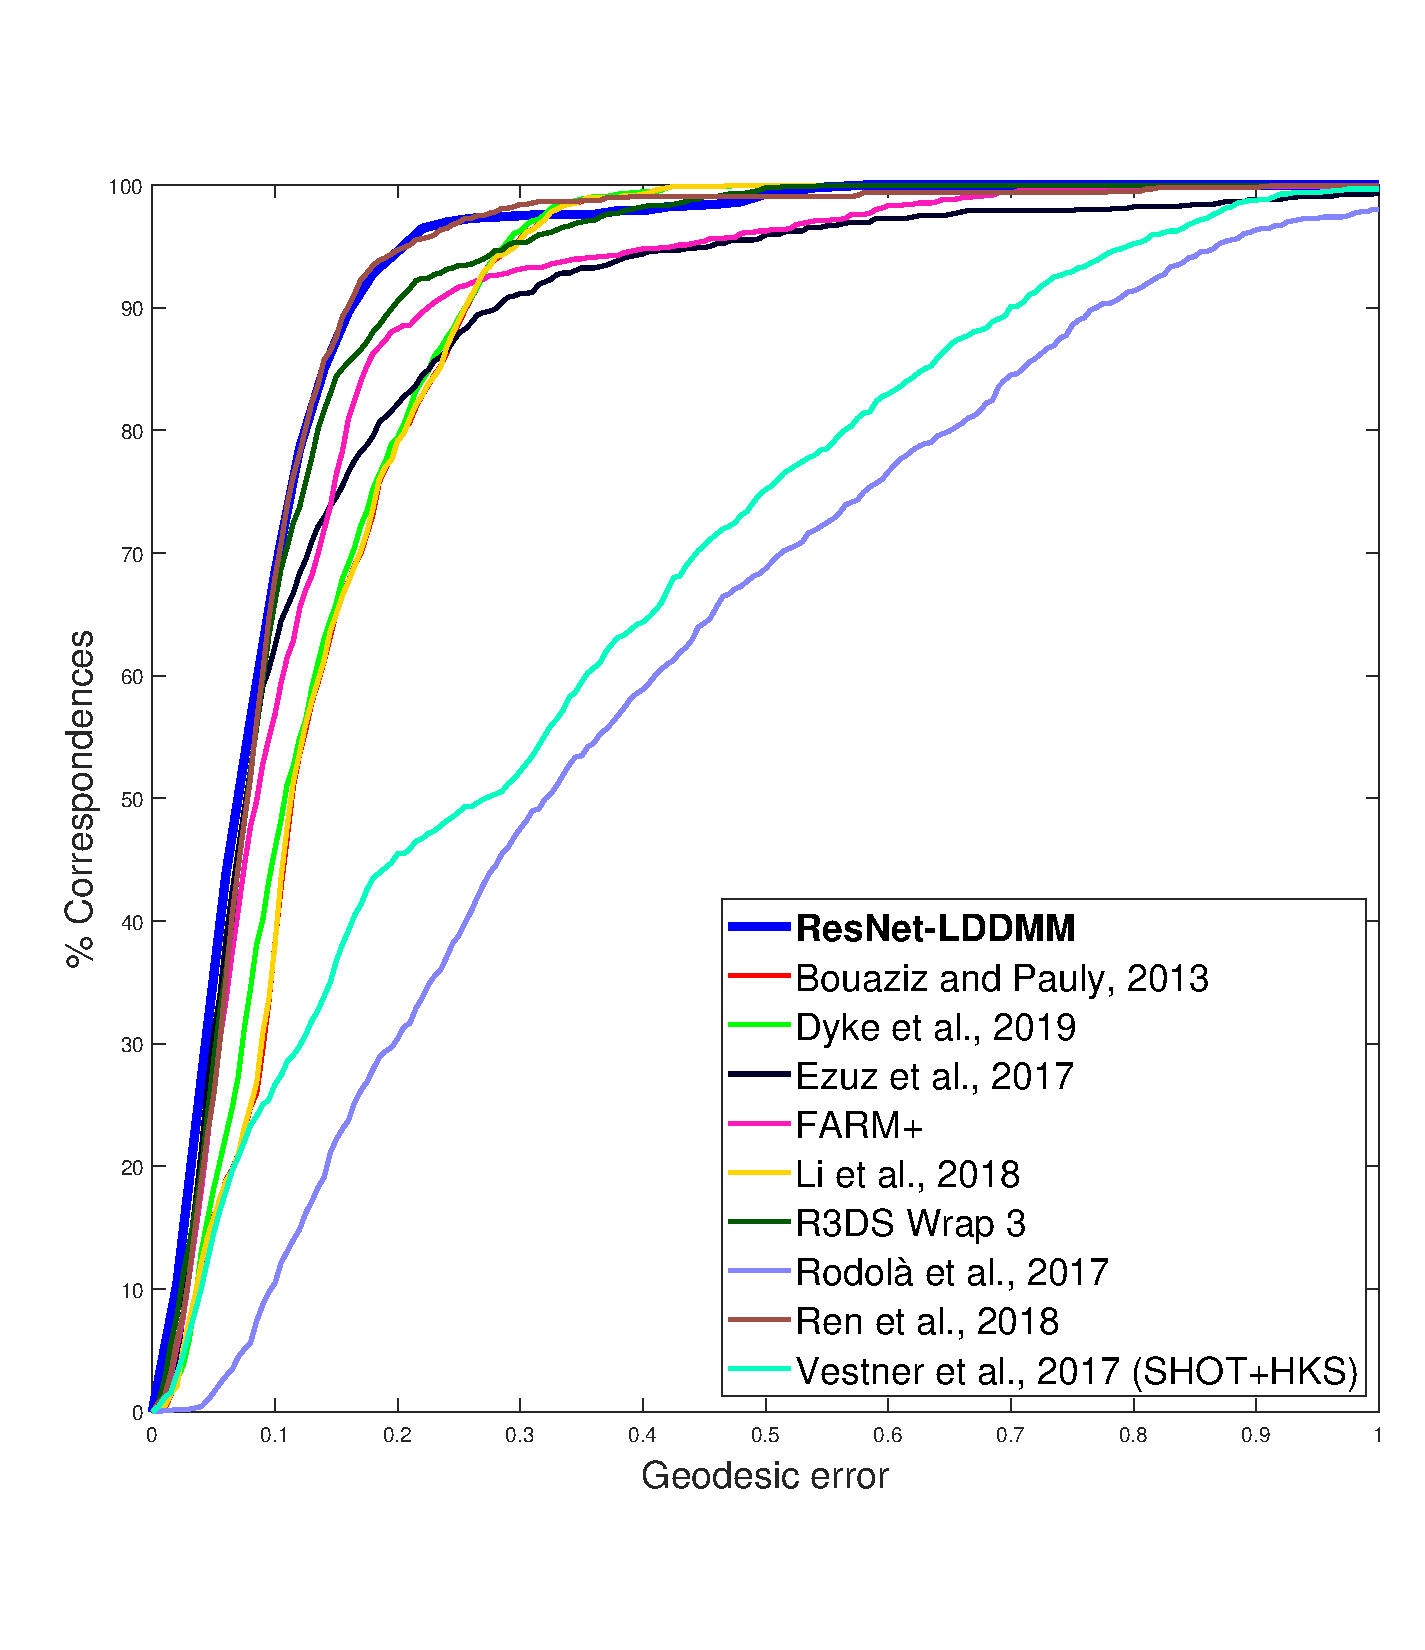
\includegraphics[width=0.19\linewidth]{Figs/7c.pdf}
    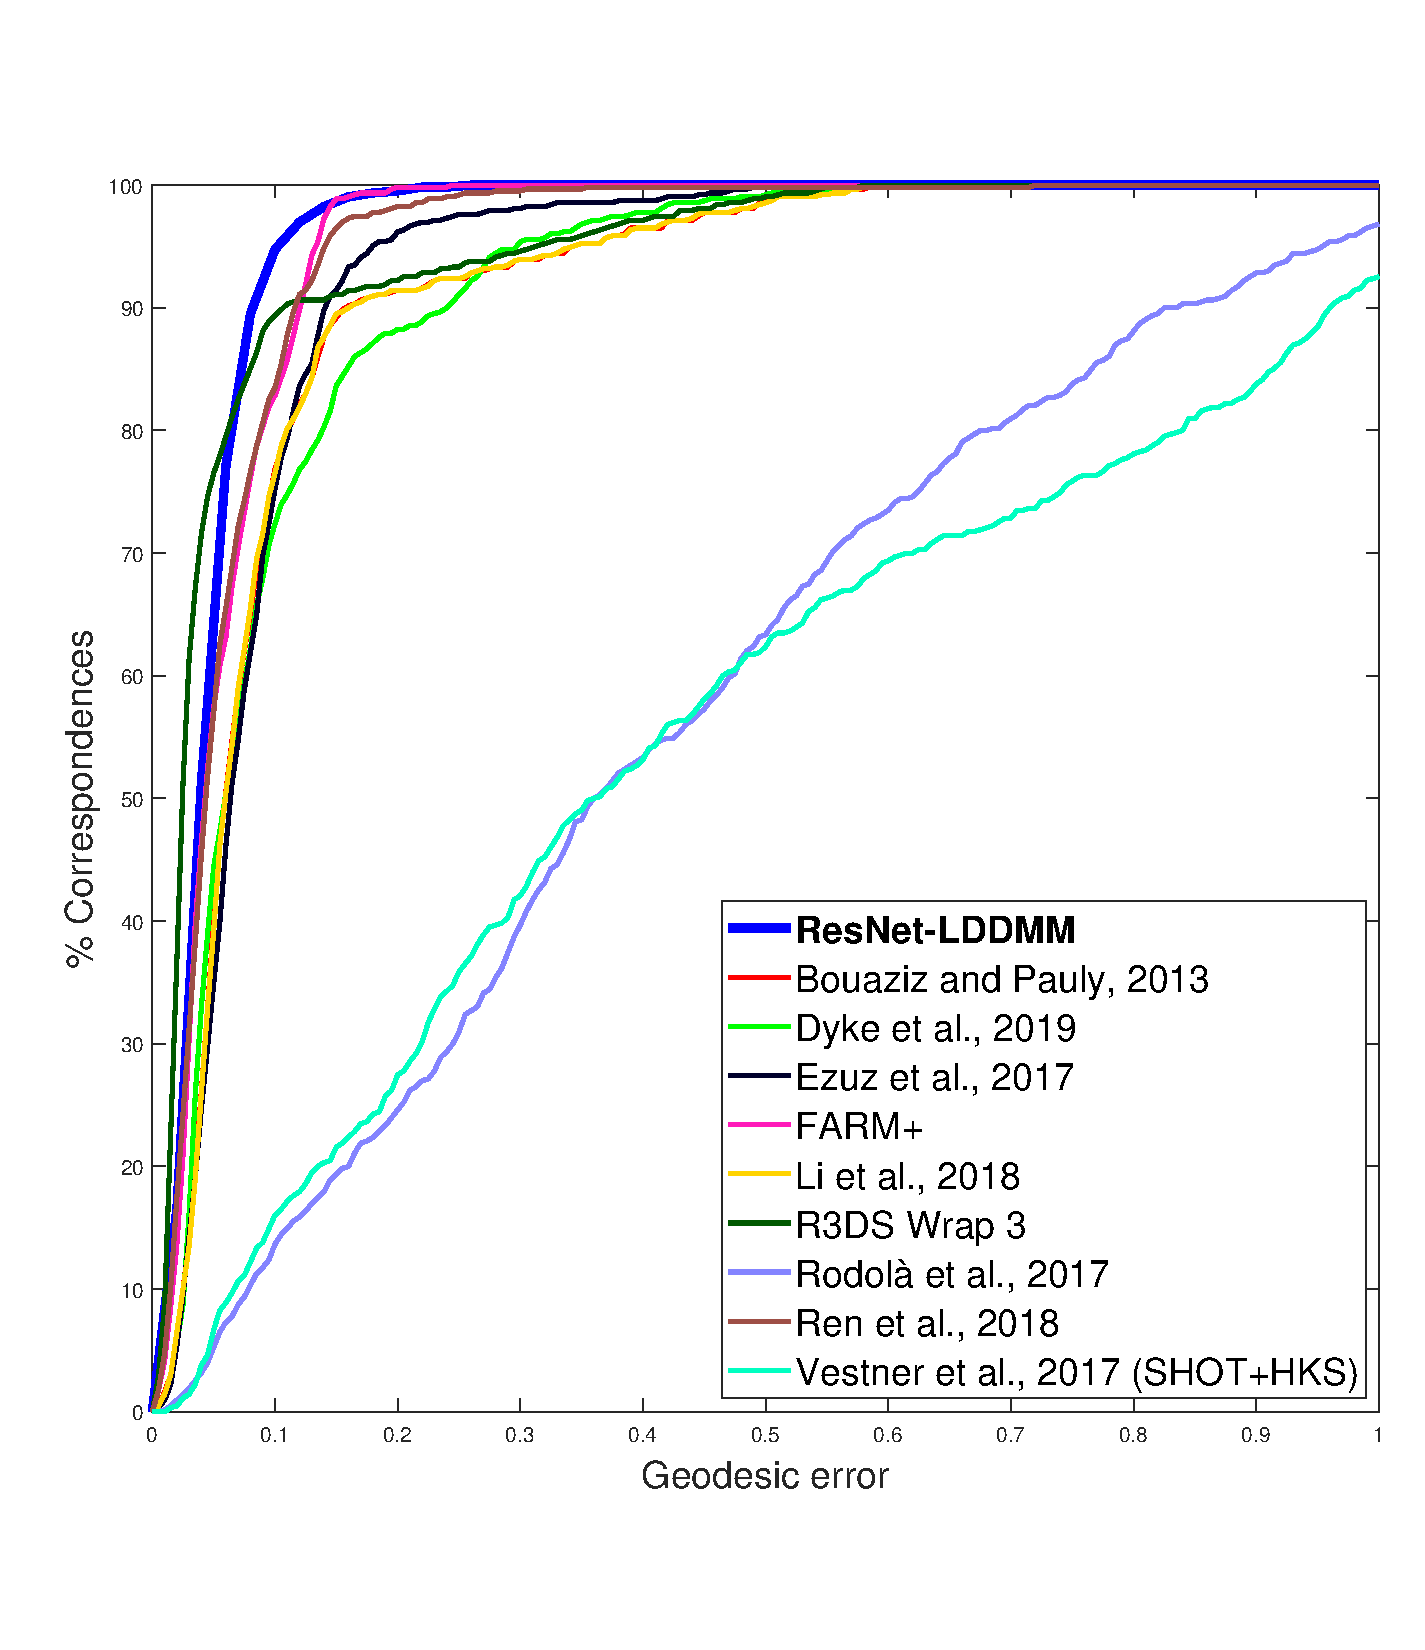
\includegraphics[width=0.19\linewidth]{Figs/7d.pdf}
    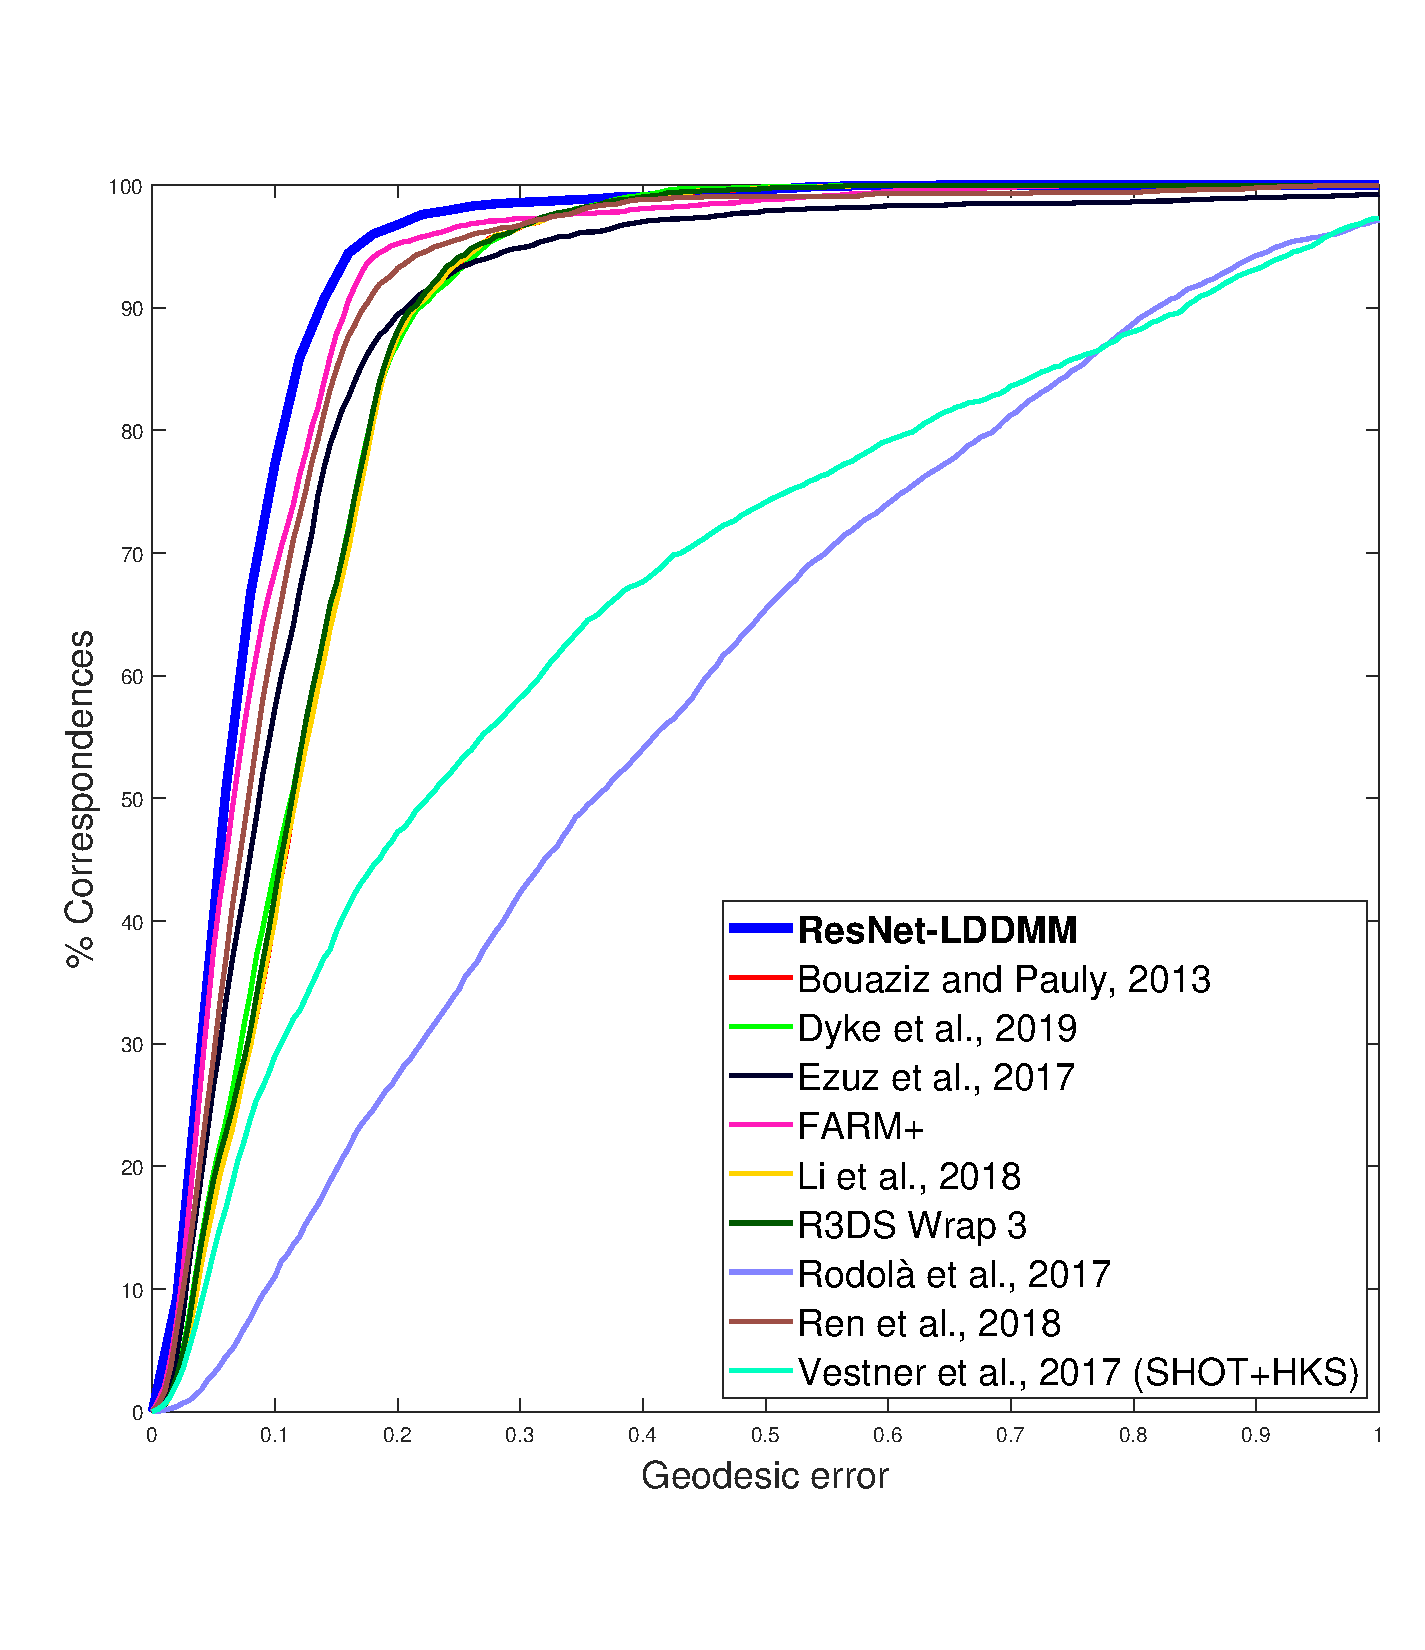
\includegraphics[width=0.19\linewidth]{Figs/9.pdf}
    \vspace{-0.3cm}
\caption{Quantitative evaluation (Geodesic Error Curves) on SHREC'2020 and comparison with existing approaches including variants of the \textit{Functional Maps} framework, as reported in \cite{dyke2020shrec}. Considered poses/deformations, from left to right: twist, indent, inflate, stretch, and overall.}
   \label{Fig:SHREC2020}
\end{figure*}

The evaluation on test-set0 revealed another limitation of our ResNet-LDDMM. For example, when the hand's fingers are close to each others in the source shape and far in the target shape, ResNet-LDDMM fails to find the correct space partition in which affine transformations are computed. This dictates the need to incorporate the mesh connectivity in the current framework. That is only neighboring connected vertices could moves together to similar directions. In this experiment, prior to shape registration using our ResNet-LDDMM, we apply a Laplacian filtering on both source and target shapes. Empirically, we found that such pre-processing helps ResNet-LDDMM to find better registration solutions. We have used the simple nearest neighbor criterion to return the final correspondence after performing our ResNet-LDDMM algorithm.

\subsection{Experiments on SHREC'2020}
\label{Sec:SHREC2020}

We have also conducted experiments on the SHREC'2020 dataset (Task.1 \cite{dyke2020shrec}). Here, the dataset contains 11 partial scans and one full scan of a rabbit toy. Each scan represents a unique combination of pose (twist, indent, inflate or stretch) and internal materials (couscous, risotto, and chickpea). The challenge consists in registering each of the partial scans with the full (neutral pose) 3D scan. Unlike the Functional Maps framework which requires an adaptation as described in \cite{rodola2017partial}, the same implementation of ResNet-LDDMM was used to register partial scans to full scans. Unlike the previous SHREC'2019 contest, all participants have reported dense correspondence results. The graphs of Fig.\ref{Fig:SHREC2020} reports quantitative results and compares ResNet-LDDMM to existing approaches. Clearly on SHREC'2020, our approach outperforms all existing methods under all deformations and filling materials. In particular, it outperforms all variants of \textit{Functional Maps} with partial matching adaptation \cite{rodola2017partial}, with denoising by blurring the map \cite{ezuz2017deblurring} and the commercial product FARM+ dedicated to 3D human bodies, grounding on the Functional Maps framework \cite{ovsjanikov2012functional}. The key point is that \textit{Functional Maps} approaches works well on near-isometric deformations and suppose clean meshes (without noise or holes). ResNet-LDDMM tolerates such imperfections, works in partial matching and handles better non-isometric transformations (\eg stretching). To sum up, these results (graphs of Fig.\ref{Fig:SHREC2019} and Fig.\ref{Fig:SHREC2020}) show clearly that ResNet-LDDMM (1) tolerates noisy and missing data caused by self-occlusion or due to partial scans as it is works on point clouds and not meshes (more results and comparisons are reported in Supplementary Materials); (2) allows to go beyond near-isometric transformations and accounts for anisotropic deformations as twist, indent, inflate, and stretch. These evaluations reflects as well some limitations of ResNet-LDDMM which are (1) the restriction of ResNet-LDDMM to compute topology-preserving transformations (\ie diffeomorphic transformations) which do not allow accurate registration of meshes with different topologies; (2) the need to incorporate initial correspondences and points connectivity, when available, in order to better guide a correct division of the space into polytopes. Limitations and strengths to use diffeomorphisms (in LDDMM family of approaches) are discussed in the next paragraph.


\subsection{The Pros and Cons of using Diffeomorphisms}
\label{Sec:limitations}
While our approach differs from the usual LDDMM framework on a few points, it preserves a key aspect of these methods: it computes a full diffeomorphism of $\R^3$, and the template and target shapes themselves only appear in the loss function. This comes with both pros and cons, both also present in the original LDDMM methods, which we will now discuss.

%\textbf{--} Because of the extrinsic nature of the network, it is not invariant by rotation or translation. 
\textbf{--} The main limitation of ResNet-LDDMM is that it will give poor result when trying to match shapes that are not topologically the same as embedded surfaces of $\R^3$. This is particularly visible when studying various poses of a hand or body: if two different parts of either shape touch in one case but not in the other (e.g., going from a closed hand to one pointing a finger), it is almost impossible to find an adequate diffeomorphism (examples reported in Fig.\ref{Fig:TopologyExamples}). The effect of this qualitative statement is shown quantitatively in Section \ref{Sec:SHREC2019} where we apply our algorithm to the SHREC'2019 database to mixed results, and visualized in Fig.\ref{Fig:TopologyExamples}. In such cases, methods that use an intrinsic approach, like Functional Maps, will perform better. 

\textbf{--} It should be noted that, depending on the goal, this ``drawback" can actually be a feature: a lot of applications of LDDMMs in computational anatomy come from its power to quantitatively tell how far one shape is from another, in addition to just matching them. This is reflected by how big the minimal value of the cost function is for various targets. In such cases, targets that are topologically different should indeed be considered very different, hence it being hard for them to be matched (see for example \cite{miller2007lddmm}).

\textbf{--} On the other hand, the well-known advantage of using diffeomorphisms is that when the shapes can be matched, it automatically ignores all transformations that do change the topology, preventing any unnecessary crossings in the shape. Moreover, because of the regularity of the transformation, it is generally very resistant to noise in the target shape. This has actually been used as a de-noising method for medical databases \cite{tward2013lddmm} (see also Fig.7 in the supplementary material). It also tolerates some missing data (see Fig.8 in the supplementary material for illustrations.

\textbf{--} Another perk of all LDDMM type methods, including ResNet-LDDMM, is that, since we obtain a diffeomorphism of all of $\R^3$, once trained, the networks can be applied to any point in the ambient space. This means that we can apply the trained transformation to a completely different parametrization of the shape. Consequently, it is possible to train the network on shapes with lowered resolutions and still get a good match for the original shapes.